% !TeX spellcheck = russian-aot-ieyo
% Зачем: Определяет класс документа (То, как будет выглядеть документ)
% Примечание: параметр draft помечает строки, вышедшие за границы страницы, прямоугольником, в фильной версии его нужно удалить.
\documentclass[a4paper,14pt,russian,oneside,final]{extreport}

% Зачем: Настройка Times New Roman.
% Рекомендовано для Windows (нужен PSCyr, подробности см. в fonts_windows.tex)
% раскомментировать, чтобы использовать:
%% Зачем: Предоставляет проприетарный Times New Roman.
% ОБНОВЛЕНИЕ: лучше использовать scalable-cyrfonts-tex: меньше проблем с установкой
% Из руководства к PSCyr: "Во избежание проблем пакет PSCyr должен загружаться перед пакета-ми inputenc и babel".
% Примечание: Требует шаманства при установке, инструкция http://plumbum-blog.blogspot.com/2010/06/miktex-28-pscyr-04d.html
% http://blog.harrix.org/?p=444
\usepackage{pscyr}

% Зачем: Выбор внутренней TeX кодировки.
\usepackage[T2A]{fontenc}

% не забудьте закомментировать % Зачем: Выбор внутренней TeX кодировки.
\usepackage[T2A]{fontenc}

% Зачем: Предоставляет свободный Times New Roman.
% Шрифт идёт вместе с пакетом scalable-cyrfonts-tex в Ubuntu/Debian

% пакет scalable-cyrfonts-tex может конфликтовать с texlive-fonts-extra в Ubuntu
% решение: Для себя я решил эту проблему так: пересобрал пакет scalable-cyrfonts-tex, изменив его имя. Решение топорное, но работает. Желающие могут скачать мой пакет здесь:
% https://yadi.sk/d/GW2PhDgEcJH7m
% Установка:
% dpkg -i scalable-cyrfonts-tex-shurph_4.16_all.deb

\usefont{T2A}{ftm}{m}{sl}


% Рекомендовано для Linux (нужен scalable-cyrfonts-tex, подробности см. в fonts_linux.tex)
% раскомментировать, чтобы использовать:
% Зачем: Выбор внутренней TeX кодировки.
\usepackage[T2A]{fontenc}

% Зачем: Предоставляет свободный Times New Roman.
% Шрифт идёт вместе с пакетом scalable-cyrfonts-tex в Ubuntu/Debian

% пакет scalable-cyrfonts-tex может конфликтовать с texlive-fonts-extra в Ubuntu
% решение: Для себя я решил эту проблему так: пересобрал пакет scalable-cyrfonts-tex, изменив его имя. Решение топорное, но работает. Желающие могут скачать мой пакет здесь:
% https://yadi.sk/d/GW2PhDgEcJH7m
% Установка:
% dpkg -i scalable-cyrfonts-tex-shurph_4.16_all.deb

\usefont{T2A}{ftm}{m}{sl}
% не забудьте закомментировать % Зачем: Предоставляет проприетарный Times New Roman.
% ОБНОВЛЕНИЕ: лучше использовать scalable-cyrfonts-tex: меньше проблем с установкой
% Из руководства к PSCyr: "Во избежание проблем пакет PSCyr должен загружаться перед пакета-ми inputenc и babel".
% Примечание: Требует шаманства при установке, инструкция http://plumbum-blog.blogspot.com/2010/06/miktex-28-pscyr-04d.html
% http://blog.harrix.org/?p=444
\usepackage{pscyr}

% Зачем: Выбор внутренней TeX кодировки.
\usepackage[T2A]{fontenc}



% Зачем: Установка кодировки исходных файлов.
\usepackage[utf8]{inputenc}

% Зачем: Делает результирующий PDF "searchable and copyable".
\usepackage{cmap}

% Зачем: Чтобы можно было использовать русские буквы в формулах, но в случае использования предупреждать об этом.
\usepackage[warn]{mathtext}

% Зачем: Учет особенностей различных языков.
\usepackage[russian]{babel}

% Зачем: Добавляет поддержу дополнительных размеров текста 8pt, 9pt, 10pt, 11pt, 12pt, 14pt, 17pt, and 20pt.
% Почему: Пункт 2.1.1 Требований по оформлению пояснительной записки.
\usepackage{extsizes}


% Зачем: Длинна, пимерно соответвующая 5 символам
% Почему: Требования содержат странное требование про отсупы в 5 символов (для немоноширинного шрифта :| )
\newlength{\fivecharsapprox}
\setlength{\fivecharsapprox}{6ex}


% Зачем: Добавляет отступы для абзацев.
% Почему: Пункт 2.1.3 Требований по оформлению пояснительной записки.
\usepackage{indentfirst}
\setlength{\parindent}{\fivecharsapprox} % Примерно соответсвует 5 символам.


% Зачем: Настраивает отступы от границ страницы.
% Почему: Пункт 2.1.2 Требований по оформлению пояснительной записки.
\usepackage[left=3cm,top=2.0cm,right=1.5cm,bottom=2.7cm]{geometry}


% Зачем: Настраивает межстрочный интервал, для размещения 40 +/- 3 строки текста на странице.
% Почему: Пункт 2.1.1 Требований по оформлению пояснительной записки.
\usepackage[nodisplayskipstretch]{setspace}
\setstretch{1.1}
%\onehalfspacing

% Зачем: Выбор шрифта по-умолчанию.
% Почему: Пункт 2.1.1 Требований по оформлению пояснительной записки.
% Примечание: В требованиях не указан, какой именно шрифт использовать. По традиции используем TNR.
\renewcommand{\rmdefault}{ftm} % Times New Roman


% Зачем: Отключает использование изменяемых межсловных пробелов.
% Почему: Так не принято делать в текстах на русском языке.
\frenchspacing


% Зачем: Сброс счетчика сносок для каждой страницы
% Примечание: в "Требованиях по оформлению пояснительной записки" не указано, как нужно делать, но в других БГУИРовских докуметах рекомендуется нумерация отдельная для каждой страницы
\usepackage{perpage}
\MakePerPage{footnote}


% Зачем: Добавляет скобку 1) к номеру сноски
% Почему: Пункты 2.9.2 и 2.9.1 Требований по оформлению пояснительной записки.
\makeatletter
\def\@makefnmark{\hbox{\@textsuperscript{\normalfont\@thefnmark)}}}
\makeatother


% Зачем: Расположение сносок внизу страницы
% Почему: Пункт 2.9.2 Требований по оформлению пояснительной записки.
\usepackage[bottom]{footmisc}


% Зачем: Переопределяем стандартную нумерацию, т.к. в отчете будут только section и т.д. в терминологии TeX
\makeatletter
\renewcommand{\thesection}{\arabic{section}}
\makeatother


% Зачем: Пункты (в терминологии требований) в терминологии TeX subsubsection должны нумероваться
% Почему: Пункт 2.2.3 Требований по оформлению пояснительной записки.
\setcounter{secnumdepth}{3}


% Зачем: Настраивает отступ между таблицей с содержанимем и словом СОДЕРЖАНИЕ
% Почему: Пункт 2.2.7 Требований по оформлению пояснительной записки.
\usepackage{tocloft}
\setlength{\cftbeforetoctitleskip}{-1em}
\setlength{\cftaftertoctitleskip}{1em}


% Зачем: Определяет отступы слева для записей в таблице содержания.
% Почему: Пункт 2.2.7 Требований по оформлению пояснительной записки.
\makeatletter
\renewcommand{\l@section}{\@dottedtocline{1}{0.5em}{1.2em}}
\renewcommand{\l@subsection}{\@dottedtocline{2}{1.7em}{2.0em}}
\makeatother


% Зачем: Работа с колонтитулами
\usepackage{fancyhdr} % пакет для установки колонтитулов
\pagestyle{fancy} % смена стиля оформления страниц


% Зачем: Нумерация страниц располагается справа снизу страницы
% Почему: Пункт 2.2.8 Требований по оформлению пояснительной записки.
\fancyhf{} % очистка текущих значений
\fancyfoot[R]{\thepage} % установка верхнего колонтитула
\renewcommand{\footrulewidth}{0pt} % убрать разделительную линию внизу страницы
\renewcommand{\headrulewidth}{0pt} % убрать разделительную линию вверху страницы
\fancypagestyle{plain}{
    \fancyhf{}
    \rfoot{\thepage}}


% Зачем: Задает стиль заголовков раздела жирным шрифтом, прописными буквами, без точки в конце
% Почему: Пункты 2.1.1, 2.2.5, 2.2.6 и ПРИЛОЖЕНИЕ Л Требований по оформлению пояснительной записки.
\makeatletter
\renewcommand\section{%
  \clearpage\@startsection {section}{1}%
    {\fivecharsapprox}%
    {-1em \@plus -1ex \@minus -.2ex}%
    {1em \@plus .2ex}%
    {\raggedright\hyphenpenalty=10000\normalfont\large\bfseries\MakeUppercase}}
\makeatother


% Зачем: Задает стиль заголовков подразделов
% Почему: Пункты 2.1.1, 2.2.5 и ПРИЛОЖЕНИЕ Л Требований по оформлению пояснительной записки.
\makeatletter
\renewcommand\subsection{%
  \@startsection{subsection}{2}%
    {\fivecharsapprox}%
    {-1em \@plus -1ex \@minus -.2ex}%
    {1em \@plus .2ex}%
    {\raggedright\hyphenpenalty=10000\normalfont\normalsize\bfseries}}
\makeatother


% Зачем: Задает стиль заголовков пунктов
% Почему: Пункты 2.1.1, 2.2.5 и ПРИЛОЖЕНИЕ Л Требований по оформлению пояснительной записки.
\makeatletter
\renewcommand\subsubsection{
  \@startsection{subsubsection}{3}%
    {\fivecharsapprox}%
    {-1em \@plus -1ex \@minus -.2ex}%
    {\z@}%
    {\raggedright\hyphenpenalty=10000\normalfont\normalsize\bfseries}}
\makeatother

% Зачем: для оформления введения и заключения, они должны быть выровнены по центру.
% Почему: Пункты 1.1.15 и 1.1.11 Требований по оформлению пояснительной записки.
\makeatletter
\newcommand\sectioncentered{%
  \clearpage\@startsection {section}{1}%
    {\z@}%
    {-1em \@plus -1ex \@minus -.2ex}%
    {1em \@plus .2ex}%
    {\centering\hyphenpenalty=10000\normalfont\large\bfseries\MakeUppercase}%
    }
\makeatother



% Зачем: Задает стиль библиографии
% Почему: Пункт 2.8.6 Требований по оформлению пояснительной записки.
\bibliographystyle{styles/belarus-specific-utf8gost780u}


% Зачем: Пакет для вставки картинок
% Примечание: Объяснение, зачем final - http://tex.stackexchange.com/questions/11004/why-does-the-image-not-appear
\usepackage[final]{graphicx}
\DeclareGraphicsExtensions{.pdf,.png,.jpg,.eps}


% Зачем: Директория в которой будет происходить поиск картинок
\graphicspath{{figures/}}


% Зачем: Добавление подписей к рисункам
\usepackage[nooneline]{caption}
\usepackage{subcaption}

% Зачем: чтобы работала \No в новых латехах
\DeclareRobustCommand{\No}{\ifmmode{\nfss@text{\textnumero}}\else\textnumero\fi}

% Зачем: поворот ячеек таблиц на 90 градусов
\usepackage{rotating}
\DeclareRobustCommand{\povernut}[1]{\begin{sideways}{#1}\end{sideways}}


% Зачем: когда в формулах много кириллических символов команда \text{} занимает много места
\DeclareRobustCommand{\x}[1]{\text{#1}}


% Зачем: Задание подписей, разделителя и нумерации частей рисунков
% Почему: Пункт 2.5.5 Требований по оформлению пояснительной записки.
\DeclareCaptionLabelFormat{stbfigure}{Рисунок #2}
\DeclareCaptionLabelFormat{stbtable}{Таблица #2}
\DeclareCaptionLabelSeparator{stb}{~--~}
\captionsetup{labelsep=stb}
\captionsetup[figure]{labelformat=stbfigure,justification=centering}
\captionsetup[table]{labelformat=stbtable,justification=raggedright}
\renewcommand{\thesubfigure}{\asbuk{subfigure}}

% Зачем: Окружения для оформления формул
% Почему: Пункт 2.4.7 требований по оформлению пояснительной записки и специфические требования различных кафедр
% Пример использования смотри в course_content.tex, строка 5
\usepackage{calc}
\newlength{\lengthWordWhere}
\settowidth{\lengthWordWhere}{где}
\newenvironment{explanationx}
    {%
    %%% Следующие строки определяют специфические требования разных редакций стандартов. Раскоменнтируйте нужную строку
    %% стандартный абзац, СТП-01 2010
    %\begin{itemize}[leftmargin=0cm, itemindent=\parindent + \lengthWordWhere + \labelsep, labelsep=\labelsep]
    %% без отступа, СТП-01 2013
    \begin{itemize}[leftmargin=0cm, itemindent=\lengthWordWhere + \labelsep , labelsep=\labelsep]%
    \renewcommand\labelitemi{}%
    }
    {%
    %\\[\parsep]
    \end{itemize}
    }

% Старое окружение для "где". Сохранено для совместимости
\usepackage{tabularx}

\newenvironment{explanation}
    {
    %%% Следующие строки определяют специфические требования разных редакций стандартов. Раскоменнтируйте нужные 2 строки
    %% стандартный абзац, СТП-01 2010
    %\par
    %\tabularx{\textwidth-\fivecharsapprox}{@{}ll@{ --- } X }
    %% без отступа, СТП-01 2013
    \noindent
    \tabularx{\textwidth}{@{}ll@{ --- } X }
    }
    {
    \\[\parsep]
    \endtabularx
    }


% Зачем: Удобная вёрстка многострочных формул, масштабирующийся текст в формулах, формулы в рамках и др
\usepackage{amsmath}


% Зачем: Поддержка ажурного и готического шрифтов
\usepackage{amsfonts}


% Зачем: amsfonts + несколько сотен дополнительных математических символов
\usepackage{amssymb}


% Зачем: Окружения «теорема», «лемма»
\usepackage{amsthm}


% Зачем: Производить арифметические операции во время компиляции TeX файла
\usepackage{calc}

% Зачем: Производить арифметические операции во время компиляции TeX файла
\usepackage{fp}

% Зачем: Пакет для работы с перечислениями
\usepackage{enumitem}
\makeatletter
 \AddEnumerateCounter{\asbuk}{\@asbuk}{щ)}
\makeatother


% Зачем: Устанавливает символ начала простого перечисления
% Почему: Пункт 2.3.5 Требований по оформлению пояснительной записки.
\setlist{nolistsep}


% Зачем: Устанавливает символ начала именованного перечисления
% Почему: Пункт 2.3.8 Требований по оформлению пояснительной записки.
\renewcommand{\labelenumi}{\asbuk{enumi})}
\renewcommand{\labelenumii}{\arabic{enumii})}

% Зачем: Устанавливает отступ от границы документа до символа списка, чтобы этот отступ равнялся отступу параграфа
% Почему: Пункт 2.3.5 Требований по оформлению пояснительной записки.

\setlist[itemize,0]{itemindent=\parindent + 2.2ex,leftmargin=0ex,label=--}
\setlist[enumerate,1]{itemindent=\parindent + 2.7ex,leftmargin=0ex}
\setlist[enumerate,2]{itemindent=\parindent + \parindent - 2.7ex}

% Зачем: Включение номера раздела в номер формулы. Нумерация формул внутри раздела.
\AtBeginDocument{\numberwithin{equation}{section}}

% Зачем: Включение номера раздела в номер таблицы. Нумерация таблиц внутри раздела.
\AtBeginDocument{\numberwithin{table}{section}}

% Зачем: Включение номера раздела в номер рисунка. Нумерация рисунков внутри раздела.
\AtBeginDocument{\numberwithin{figure}{section}}


% Зачем: Дополнительные возможности в форматировании таблиц
\usepackage{makecell}
\usepackage{multirow}
\usepackage{array}


% Зачем: "Умная" запятая в математических формулах. В дробных числах не добавляет пробел
% Почему: В требованиях не нашел, но в русском языке для дробных чисел используется {,} а не {.}
\usepackage{icomma}

% Зачем: макрос для печати римских чисел
\makeatletter
\newcommand{\rmnum}[1]{\romannumeral #1}
\newcommand{\Rmnum}[1]{\expandafter\@slowromancap\romannumeral #1@}
\makeatother


% Зачем: Управление выводом чисел.
\usepackage{sistyle}
\SIdecimalsign{,}

% Зачем: inline-коментирование содержимого.
\newcommand{\ignore}[2]{\hspace{0in}#2}


% Зачем: Возможность коментировать большие участки документа
\usepackage{verbatim}


\usepackage{xcolor}


% Зачем: Оформление листингов кода
% Примечание: final нужен для переопределения режима draft, в котором листинги не выводятся в документ.
\usepackage[final]{listings}


% Зачем: настройка оформления листинга для языка F#
\definecolor{bluekeywords}{rgb}{0.13,0.13,1}
\definecolor{greencomments}{rgb}{0,0.5,0}
\definecolor{turqusnumbers}{rgb}{0.17,0.57,0.69}
\definecolor{redstrings}{rgb}{0.5,0,0}

\renewcommand{\lstlistingname}{Листинг}

\lstdefinelanguage{FSharp}
    {morekeywords={abstract,and,as,assert,base,begin,class,default,delegate,do,done,downcast,downto,elif,else,end,exception,extern,false,finally,for,fun,function,global,if,in,inherit,inline,interface,internal,lazy,let,let!,match,member,module,mutable,namespace,new,not,null,of,open,or,override,private,public,rec,return,return!,select,static,struct,then,to,true,try,type,upcast,use,use!,val,void,when,while,with,yield,yield!,asr,land,lor,lsl,lsr,lxor,mod,sig,atomic,break,checked,component,const,constraint,constructor,continue,eager,event,external,fixed,functor,include,method,mixin,object,parallel,process,protected,pure,sealed,tailcall,trait,virtual,volatile},
    keywordstyle=\bfseries\color{bluekeywords},
    sensitive=false,
    morecomment=[l][\color{greencomments}]{///},
    morecomment=[l][\color{greencomments}]{//},
    morecomment=[s][\color{greencomments}]{{(*}{*)}},
    morestring=[b]",
    stringstyle=\color{redstrings},
    }

\lstdefinestyle{fsharpstyle}{
   xleftmargin=0ex,
   language=FSharp,
   basicstyle=\footnotesize\ttfamily,
   breaklines=true,
   columns=fullflexible
}

\lstdefinestyle{csharpinlinestyle} {
  language=[Sharp]C,
  morekeywords={yield,var,get,set,from,select,partial,where,async,await},
  breaklines=true,
  columns=fullflexible,
  basicstyle=\footnotesize\ttfamily
}

\lstdefinestyle{csharpstyle}{
  language=[Sharp]C,
  frame=lr,
  rulecolor=\color{blue!80!black}}


\lstdefinelanguage{JavaScript}{
  morekeywords={typeof, new, true, false, catch, function, return, null, catch, switch, var, if, in, while, do, else, case, break},
  morecomment=[s]{/*}{*/},
  morecomment=[l]//,
  morestring=[b]",
  morestring=[b]'
}

\lstdefinelanguage{HTML5}{
    language=html,
    sensitive=true,
    alsoletter={<>=-},
    otherkeywords={
    % HTML tags
    <html>, <head>, <title>, </title>, <meta, />, </head>, <body>,
    <canvas, \/canvas>, <script>, </script>, </body>, </html>, <!, html>, <style>, </style>, ><
    },
    ndkeywords={
    % General
    =,
    % HTML attributes
    charset=, id=, width=, height=,
    % CSS properties
    border:, transform:, -moz-transform:, transition-duration:, transition-property:, transition-timing-function:
    },
    morecomment=[s]{<!--}{-->},
    tag=[s]
}



% Зачем: Нумерация листингов в пределах секции
\AtBeginDocument{\numberwithin{lstlisting}{section}}

\usepackage[normalem]{ulem}

\usepackage[final,hidelinks]{hyperref}
% Моноширинный шрифт выглядит визуально больше, чем пропорциональный шрифт, если их размеры одинаковы. Искусственно уменьшаем размер ссылок.
\renewcommand{\UrlFont}{\small\rmfamily\tt}

\usepackage[square,numbers,sort&compress]{natbib}
\setlength{\bibsep}{0em}

% Магия для подсчета разнообразных объектов в документе
\usepackage{lastpage}
\usepackage{totcount}
\regtotcounter{section}

\usepackage{etoolbox}

\newcounter{totfigures}
\newcounter{tottables}
\newcounter{totreferences}
\newcounter{totequation}

\providecommand\totfig{}
\providecommand\tottab{}
\providecommand\totref{}
\providecommand\toteq{}

\makeatletter
\AtEndDocument{%
  \addtocounter{totfigures}{\value{figure}}%
  \addtocounter{tottables}{\value{table}}%
  \addtocounter{totequation}{\value{equation}}
  \immediate\write\@mainaux{%
    \string\gdef\string\totfig{\number\value{totfigures}}%
    \string\gdef\string\tottab{\number\value{tottables}}%
    \string\gdef\string\totref{\number\value{totreferences}}%
    \string\gdef\string\toteq{\number\value{totequation}}%
  }%
}
\makeatother

\pretocmd{\section}{\addtocounter{totfigures}{\value{figure}}\setcounter{figure}{0}}{}{}
\pretocmd{\section}{\addtocounter{tottables}{\value{table}}\setcounter{table}{0}}{}{}
\pretocmd{\section}{\addtocounter{totequation}{\value{equation}}\setcounter{equation}{0}}{}{}
\pretocmd{\bibitem}{\addtocounter{totreferences}{1}}{}{}



% Для оформления таблиц не влязящих на 1 страницу
\usepackage{longtable}

% Для включения pdf документов в результирующий файл
\usepackage{pdfpages}

% Для использования знака градуса и других знаков
% http://ctan.org/pkg/gensymb
\usepackage{gensymb}

% Зачем: преобразовывать текст в верхний регистр командой MakeTextUppercase
\usepackage{textcase}

% Зачем: Переносы в словах с тире.
% Тире в словае заменяем на \hyph: аппаратно\hyphпрограммный.
% https://stackoverflow.com/questions/2193307/how-to-get-latex-to-hyphenate-a-word-that-contains-a-dash#
\def\hyph{-\penalty0\hskip0pt\relax}

% Добавляем абзацный отступ для библиографии
% https://github.com/mstyura/bsuir-diploma-latex/issues/19
\setlength\bibindent{-1.0900cm}

\makeatletter
\renewcommand\NAT@bibsetnum[1]{\settowidth\labelwidth{\@biblabel{#1}}%
   \setlength{\leftmargin}{\bibindent}\addtolength{\leftmargin}{\dimexpr\labelwidth+\labelsep\relax}%
   \setlength{\itemindent}{-\bibindent+\fivecharsapprox-0.240cm}%
   \setlength{\listparindent}{\itemindent}
\setlength{\itemsep}{\bibsep}\setlength{\parsep}{\z@}%
   \ifNAT@openbib
     \addtolength{\leftmargin}{\bibindent}%
     \setlength{\itemindent}{-\bibindent}%
     \setlength{\listparindent}{\itemindent}%
     \setlength{\parsep}{10pt}%
   \fi
}

\setlength{\abovecaptionskip}{20pt plus 20pt minus 20pt}


\newcommand{\ajs}{AngularJS}
\newcommand{\ror}{Ruby on Rails}
\newcommand{\csharp}{C\#}
\newcommand{\fsharp}{F\#}
\newcommand{\vbnet}{Visual Basic~.NET}
\newcommand{\cpp}{C\texttt{\hspace{-0.3ex}+\hspace{-0.25ex}+}}
\newcommand{\cppcli}{Visual \cpp{}/CLI}
\newcommand{\dotnet}{Microsoft .NET}
\newcommand{\netfx}{.NET Framework}
\newcommand{\java}{Java}


\begin{document}

\begin{titlepage}
  \begin{center}
    Министерство образования Республики Беларусь\\[1em]
    Учреждение образования\\
    БЕЛОРУССКИЙ ГОСУДАРСТВЕННЫЙ УНИВЕРСИТЕТ \\
    ИНФОРМАТИКИ И РАДИОЭЛЕКТРОНИКИ\\[1em]

    \begin{minipage}{\textwidth}
      \begin{flushleft}
        \begin{tabular}{ l l }
          Факультет & Компьютерных систем и сетей\\
          Кафедра   & Информатики
        \end{tabular}
      \end{flushleft}
    \end{minipage}\\[1em]

    \begin{flushright}
      \begin{minipage}{0.4\textwidth}
        \textit{К защите допустить:}\\[0.8em]
        Заведующая кафедрой информатики\\[0.45em]
        \underline{\hspace*{2.8cm}} Н.\,А.~Волорова
      \end{minipage}\\[2.2em]
    \end{flushright}

    %%
    %% ВНИМАНИЕ: на некторых факультетах (ФКП) и кафедрах (ПИКС) слова "ПОЯСНИТЕЛЬНАЯ ЗАПИСКА" предлагается (требуется) оформлять полужирным начертанием. Раскомментируйте нужную для вас строку:
    %%
    %\textbf{ПОЯСНИТЕЛЬНАЯ ЗАПИСКА}\\
    {ПОЯСНИТЕЛЬНАЯ ЗАПИСКА}\\
    {к дипломному проекту}\\
    {на тему:}\\[1em]
    \textbf{\large СЕРВИС, ПРЕДОСТАВЛЯЮЩИЙ ВОЗМОЖНОСТЬ ПОЛУЧЕНИЯ НОВИНОК МУЗЫКАЛЬНОЙ ИНДУСТРИИ}\\[1em]


    {БГУИР ДП 1-40 04 01 00 045 ПЗ}\\[2em]

    \begin{tabular}{ p{0.65\textwidth}p{0.25\textwidth} }
      Студент & Т.\,С.~Лавник \\
      Руководитель & В.\,В.~Шиманский \\
      Консультанты: &\\
      \hspace*{3ex}\emph{от кафедры информатики} & В.\,В.~Шиманский \\
      \hspace*{3ex}\emph{по экономической части} & К.\,Р.~Литвинович \\
      Нормоконтролёр & Н.\,Н.~Бабенко\\
      & \\
      Рецензент &
    \end{tabular}

    \vfill
    {\normalsize Минск 2017}
  \end{center}
\end{titlepage}
 % page 1

\sectioncentered*{Реферат}
\thispagestyle{empty}
%%
%% ВНИМАНИЕ: этот реферат не соответствует СТП-01 2013
%% пример оформления реферата смотрите здесь: http://www.bsuir.by/m/12_100229_1_91132.docx
%%

\emph{Ключевые слова}: музыкальная публикация; артист; тип публикации; поиск артистов; отложенные задачи.

\vspace{4\parsep}

Дипломный проект выполнен на 6 листах формата А1 с пояснительной запиской на~\pageref*{LastPage} страницах, без приложений справочного или информационного характера.
Пояснительная записка включает \total{section}~глав, \totfig{}~рисунков, \tottab{}~таблиц, \toteq{}~формул и \totref{}~литературный источник.

Целью дипломного проекта является создание инструмента, позволяющего решать задачи поиска новых музыкальных публикаций удобным способом.

Для достижения цели дипломного проекта было разработано веб-приложение на фреймворке Ruby on Rails.
Веб-приложение может быть использовано для получения новых публикаций интересующих пользователя артистов.
В приложении используются алгоритмы, позволяющие периодически проверять различные сервисы на наличие обновлений, касающихся интересующих релизов артистов. Также в приложении присутствует email-рассылка, отправляемая пользователям в случае наличия обновлений.

В разделе технико"=экономического обоснования был произведён расчёт затрат на создание ПО, а также экономии средств при приобретении программного продукта, получаемой пользователем.
Проведённые расчёты показали экономическую целесообразность проекта.

\clearpage
 % page 2

%{
  \newgeometry{top=1.25cm,bottom=1.25cm,right=1cm,left=2cm,twoside}
  \thispagestyle{empty}
  \setlength{\parindent}{0em}

  \newcommand{\lineunderscore}{\uline{\hspace*{\fill}}}

  \begin{center}
    Министерство образования Республики Беларусь\\
    Учреждение образования\\
    БЕЛОРУССКИЙ ГОСУДАРСТВЕННЫЙ УНИВЕРСИТЕТ \\
    ИНФОРМАТИКИ И РАДИОЭЛЕКТРОНИКИ\\[1em]
  

  \begin{minipage}{\textwidth}
    \begin{flushleft}
      \begin{tabular}{ p{0.20\textwidth}p{0.31\textwidth}p{0.20\textwidth}p{0.20\textwidth} @{} }
        Факультет & КСиС & Кафедра & Информатики \\
        Специальность   & 1-31 03 04 & Специализация & 07
      \end{tabular}
    \end{flushleft}
  \end{minipage}\\[1em]

  \begin{minipage}{\textwidth}
    \begin{flushright}
      \begin{tabular}{p{0.40\textwidth}}
        УТВЕРЖДАЮ \\[0.5em]
        \underline{\hspace*{7em}} Зав. кафедрой \\
        <<\underline{\hspace*{4ex}}>> \underline{\hspace*{7em}} 2013 г.
      \end{tabular}
    \end{flushright}
  \end{minipage}\\[1em]

  \textbf{ЗАДАНИЕ} \\
  \textbf{по дипломному проекту (работе) студента}

  \lineunderscore \\
  {\small (фамилия, имя, отчество) }

  \end{center}

  1. Тема проекта (работы):
  \lineunderscore\\
  \lineunderscore\\
  \lineunderscore\\
  утверждена приказом по университету от \uline{\hspace*{1.5em}} \uline{\hspace*{5em}} 2013 г.  \No{} \uline{\hspace*{2em}}-с

  \vspace{1em}

  2. Срок сдачи студентом законченного проекта (работы): \lineunderscore

  \vspace{1em}

  3. Исходные данные к проекту (работе):
  \lineunderscore\\
  \lineunderscore\\
  \lineunderscore\\
  \lineunderscore\\
  \lineunderscore\\
  \lineunderscore

  \vspace{1em}

  4. Содержание пояснительной записки (перечень подлежащих разработке вопросов):
  \lineunderscore\\
  \lineunderscore\\
  \lineunderscore\\
  \lineunderscore\\
  \lineunderscore\\
  \lineunderscore\\
  \lineunderscore\\
  \lineunderscore\\
  \lineunderscore\\
  \lineunderscore\\
  \lineunderscore

  \clearpage
  \thispagestyle{empty}

  5. Перечень графического материала (с точным указанием обязательных чертежей):
  \lineunderscore\\
  \lineunderscore\\
  \lineunderscore\\
  \lineunderscore\\
  \lineunderscore\\
  \lineunderscore\\
  \lineunderscore\\
  \lineunderscore

  \vspace{1em}

  6. Содержание задания по технико-экономическому обоснованию:
  \lineunderscore\\
  \lineunderscore\\
  \lineunderscore

  Задание выдал: \hfill{} \uline{\hspace*{6em}} / И.\,О.~Фамилия /   

  \vspace{1em}

  7. Содержание задания по охране труда и экологической безопасности, ресурсо- и энергосбережению (\textit{указывается конкретное наименование раздела}): 
  \lineunderscore\\
  \lineunderscore\\
  \lineunderscore

  Задание выдал:  \hfill{} \uline{\hspace*{6em}} / И.\,О.~Фамилия /  

  \vfill

  \begin{center}
    КАЛЕНДАРНЫЙ ПЛАН
  \end{center}

  \begin{tabular}{| >{\centering}m{0.04\textwidth} 
                  | >{\centering}m{0.40\textwidth} 
                  | >{\centering}m{0.08\textwidth}
                  | >{\centering}m{0.19\textwidth}  
                  | >{\centering\arraybackslash}m{0.16\textwidth}|}
    \hline \No{} \No{} п/п & Наименование этапов дипломного проекта (работы) & Объем этапа, \% & Срок выполнения этапов & Примечание \\
    \hline & & & & \\
    \hline & & & & \\
    \hline & & & & \\
    \hline & & & & \\
    \hline & & & & \\
    \hline & & & & \\
    \hline & & & & \\
    \hline & & & & \\
    \hline & & & & \\
    \hline & & & & \\
    \hline & & & & \\
    \hline
  \end{tabular}

  \vspace{2em}

  Дата выдачи задания: \uline{\hspace*{6em}} \hspace{2ex} Руководитель \hfill{} \uline{\hspace*{4em}} / И.\,О.~Фамилия /

  \vspace{1em}

  Задание принял к исполнению \hfill{} \uline{\hspace*{4em}} / И.\,О.~Фамилия /

  \restoregeometry
} % pages 3 and 4. printed separately

\sectioncentered*{Аннотация}
\thispagestyle{empty}

\begin{center}
  \begin{minipage}{0.82\textwidth}
    на дипломный проект <<Сервис, предоставляющий возможность получения новинок музыкальной индустрии>> студента УО <<Белорусский государственный университет информатики и радиоэлектроники>> Лавник~Т.\,С.
  \end{minipage}
\end{center}

\emph{Ключевые слова}: музыкальная публикация; артист; тип публикации; поиск артистов; отложенные задачи.

\vspace{4\parsep}

Дипломный проект выполнен на 6 листах формата А1 с пояснительной запиской на~\pageref*{LastPage} страницах, без приложений справочного или информационного характера.
Пояснительная записка включает \total{section}~глав, \totfig{}~рисунков, \tottab{}~таблиц, \toteq{}~формул и \totref{}~литературный источник.

Целью дипломного проекта является создание инструмента, позволяющего решать задачи поиска новых музыкальных публикаций удобным способом.

Для достижения цели дипломного проекта было разработано веб-приложение на фреймворке Ruby on Rails.
Веб-приложение может быть использовано для получения новых публикаций интересующих пользователя артистов.
В приложении используются алгоритмы, позволяющие периодически проверять различные сервисы на наличие обновлений, касающихся интересующих релизов артистов. Также в приложении присутствует email-рассылка, отправляемая пользователям в случае наличия обновлений.

Во введении производится ознакомление с проблемой, решаемой в дипломном проекте.

В первой главе производится обзор предметной области проблемы решаемой в данном дипломном проекте.
Приводятся необходимые теоретические сведения, а также производится обзор существующих разработок.

Во второй главе производится краткий обзор технологий, использованных для реализации ПО в рамках дипломного проекта.

В третьей главе производится обзор реализованного ПО.
Описываются его составные части и особенности.
Приводятся результаты практических испытаний и производится сравнение с существующим ПО.

В четвертой главе производится технико"=экономическое обоснование разработки.

В заключении подводятся итоги и делаются выводы по дипломному проекту, а также описывается дальнейший план развития проекта.

\clearpage
 % not part of report

%% Содержимое данного документа позаимсвовано из Приложения Е из документа http://www.bsuir.by/m/12_113415_1_66883.pdf

\thispagestyle{empty}

\begin{singlespace}

{\small
  \begin{center}
    \begin{minipage}{0.8\textwidth}
      \begin{center}
        {\normalsize ОТЗЫВ}\\[1em]
        на дипломный проект студентки факультета информационных технологий 
        и управления Учреждения образования <<Белорусский государственный университет информатики и радиоэлектроники>>\\
        Москаленко Ольги Николаевны \\
        на тему: <<Система передачи данных>>
      \end{center}
    \end{minipage}
  \end{center}

На время дипломного проектирования перед студенткой Москаленко~О.\,Н. была поставлена задача разработать высокоскоростную систему передачи данных по занятым телефонным линиям.
Тема является актуальной, т.\,к. многие абоненты, имеющие дома компьютеры, для выхода на коллективные сети передачи данных имеют только телефонную линию связи, по которой могут вестись интенсивные разговоры.
Проблема <<последней мили>> при разработке высоконадежных систем передачи данных является основной при создании подобных систем.

Москаленко~О.\,Н. на основании анализа большого количества специализированной литературы произвела выбор частотного диапазона для передачи данных в обоих направлениях и предложила для повышения достоверности передачи информации применить решающую обратную связь.

В процессе проектирования были разработаны алгоритмы функционирования, структурные и принципиальные схемы.
Система разработана на современной элементной базе с использованием pic контроллеров.

Приведенные расчеты и программное обеспечение "--- это результат высокоэффективной работы над темой и умения использовать техническую литературу и применять на практике знания, полученные за годы обучения в университете.

Работа над проектом велась ритмично и в соответствии с календарным графиком.
Пояснительная записка и графический материал оформлены аккуратно и в соответствии с требованиями ЕСКД.

Результаты, полученные в дипломном проекте, использованы в разработке системы передачи дискретной информации, которая рекомендована к серийному выпуску, о чем свидетельствует Акт внедрения, прилагаемый к пояснительной записке.

Дипломный проект Москаленко~О.\,Н. соответствует техническому заданию и отличается глубокой проработкой темы и выполнен с применением современных прогрессивных технологий.

Считаю, что Москаленко~О.\,Н. освоила технику инженерного проектирования технических систем, подготовлена к самостоятельной работе по специальности 1-53~01~07
<<Информационные технологии и управление в технических системах>> и заслуживает присвоения квалификации инженера по информационным технологиям и управлению.

  \vfill
  \noindent
  \begin{minipage}{0.54\textwidth}
    \begin{flushleft}
      Руководитель проекта:\\
      д-р техн. наук, начальник сектора \\
      информационных технологий НАН Беларуси\\
      23.01.09
    \end{flushleft}
  \end{minipage}
  \begin{minipage}{0.44\textwidth}
    \begin{flushright}
      \underline{\hspace*{3cm}} М.\,Н.~Реут
    \end{flushright}
  \end{minipage}
}

\end{singlespace}

\clearpage % not part of report

%% Содержимое данного документа позаимсвовано из Приложения Ж из документа http://www.bsuir.by/m/12_113415_1_66883.pdf

\thispagestyle{empty}

\begin{singlespace}

{\small
  \begin{center}
    \begin{minipage}{0.9\textwidth}
      \begin{center}
        {\normalsize РЕЦЕНЗИЯ}\\[0.2cm]
        на дипломный проект студента факультета компьютерных систем и сетей Учреждения образования <<Белорусский государственный университет информатики и радиоэлектроники>>\\
        Радевича Сергея Ивановича \\
        на тему: <<Устройство квантово-криптографического закрытия информации>>
      \end{center}
    \end{minipage}\\
  \end{center}

Дипломный проект студента Радевича С. И. состоит из семи листов графического материала и~\pageref*{LastPage} страницы пояснительной записки.

Тема проекта является актуальной и посвящена разработке симплексной с асинхронно"=синхронным режимом передачи, с квантово"=криптографической защитой информации (данных и речи) системы передачи цифровой информации. 
Разработка данного устройства обусловлена необходимостью создания средств связи, надѐжно защищенных от несанкционированного доступа.

Пояснительная записка построена логично и последовательно отражает все этапы разработки в соответствии с календарным планом.

В пояснительной записке достаточно полно сделан обзор современных криптографических методов генерации секретного ключа, четко изложены методы генерации секретного
ключа в квантовой криптографии.
Разработаны схема продвижения информации в квантовой криптографии, конструкции передающего и принимающего устройств; выбраны источник и детектор единичных фотонов; предложен механизм, управляющий поляризацией отправляемых в канал связи фотонов, который основан на использовании биморфной пьезоэлектрической балки в качестве микроисполнительного устройства. 
Произведен выбор метода передачи двоичных сигналов, разработаны алгоритмы функционирования, схемы структурные и принципиальные.
В проекте приведен глубокий аналитический обзор научно"=технической литературы, где рассмотрены все вопросы, касающиеся темы проекта.
Приведенные расчеты и программное обеспечение свидетельствуют о глубоких знаниях студента Радевича~С.\,И. в области проектирования подобных систем, умении работать с технической литературой и применять на практике наиболее рациональные решения.

По каждому разделу и в целом по дипломному проекту приведены аргументированные выводы.

Пояснительная записка и графический материал оформлены аккуратно и в соответствии с требованиями ЕСКД.
Считаю, что представленные материалы могут быть использованы при разработке промышленных систем, а также студентами при изучении соответствующих разделов дисциплины <<Теория передачи информации>>.

Замечания:
\begin{itemize}
  \item при расчете числа строительных длин в выражении (7.1) длина регенеративного участка принята 80 км, в то же время по ТЗ расстояние передачи до 100 км;
  \item при расчете помехоустойчивости не указан тип помех, которые действуют в линии связи;
  \item при расчете узла тактовой синхронизации (с. 89) отсутствует обоснование выбора десятитактного регистра сдвига DD3.
\end{itemize}

В целом дипломный проект выполнен технически грамотно, в полном соответствии с техническим заданием на проектирование и заслуживает оценки десять баллов, а диплом
ник Радевич~С.\,И. "--- присвоения квалификации инженера по автоматическому управлению.

  \vfill
  \noindent
  \begin{minipage}{0.4\textwidth}
    \begin{flushleft}
      Рецензент:\\
      канд. техн. наук, профессор\\
      кафедры ИТАС БГУИР
    \end{flushleft}
  \end{minipage}
  \begin{minipage}{0.58\textwidth}
    \begin{flushright}
    \underline{\hspace*{3cm}}\hspace*{0.5cm}\underline{\hspace*{2cm}} М.\,П.~Ревотюк \\
    Дата\hspace*{6.5cm}
    \end{flushright}
  \end{minipage}
}

\end{singlespace}
\clearpage % not part of report

\setcounter{page}{5}

% Зачем: Содержание пишется полужирным шрифтом, по центру всеми заглавными буквами
% Почему: Пункт 2.2.7 Требований по оформлению пояснительной записки.
\renewcommand \contentsname {\centerline{\bfseries\large{\MakeUppercase{содержание}}}}

% Зачем: Не захламлять основной файл
% Примечание: \small\selectfont злостный хак, чтобы уменьшить размер шрифта в ToC 
{
\normalsize\selectfont
\tableofcontents
\newpage
}

\sectioncentered*{Введение}
\addcontentsline{toc}{section}{Введение}
\label{sec:intro}

Музыка сопровождала человечество на протяжении всей истории. Вначале люди использовали только свой голос, потом появились музыкальные инструменты. До сих пор прогресс не стоит на месте. С появлением компьютерной техники и интернета появилось ещё больше возможностей для самовыражения: программное обеспечение для звукозаписи, веб-сайты для публикации своих произведений, сервисы для анализа предпочтений и тому подобное. Учитывая существование изобилия музыкальных ресурсов, которые предоставлют пользователям разнообразные возможности, становится трудно следить за новыми публикациями любимых исполнителей, и, хотя подобные сервисы уже присутствуют на мировом рынке, не все они являются удобными и логически законченными.

В связи с вышесказанным, целью данного диплома является создание сервиса, который будет предоставлять возможность удобного получения уведомлений о новинках музыкальной индустрии. Сервис должен быть оснащён понятным и дружелюбным интерфейсом, позволять пользователю удобно регистрироваться и наполнять данными свой профиль, указывая свои предпочтения в виде списка интересующих артистов.

Для того, чтобы сервис был полезен пользователю, он должен быть удобен, привлекателен и реализовывать некоторую потребность. В этом состоит основа данного дипломного проекта: собирать информацию из разных сервисов в одном месте, тем самым упрощая этот для конечного пользователя. В некотором роде - это агрегат, который собирает интересы и возвращает ответ в виде удовлетворения этих интересов путём указания ссылок на публикации любимых артистов. Удобство должно быть выражено в дизайне интерфейса, который должен быть интуитивно ясен пользователю и помогать ему производить некоторые операции внутри сервиса. Также проект должен быть хорошо масштабируемым, чтобы можно было легко добавлять разные источники публикаций в свой арсенал.

Дипломный проект выполнен самостоятельно, проверен в системе «Атиплагиат». Процент оригинальности соответствует норме, установленной кафедрой информатики. Цитирования обозначены ссылками на публикации, указанные в разделе «Список использованных источников».


\section{Обзор предметной области}
\label{sec:domain}

\subsection{Постановка задачи}
\label{sub:domain:problem_formulation}
Целью данного дипломного проекта является создание веб-сервиса, состоящего из серверной и клиентской частей с использованием фреймворков Ruby on Rails~\cite{rails_guides}, AngularJS~\cite{angularjs_doc}, Sidekiq~\cite{sidekiq_doc}, для получения уведомлений о новинках в музыкальной индустрии.

Для реализации данного проекта можно выделить следующие минимальные требования:

\begin{itemize}
  \item Система должна быть компонентной, то есть разделенной на отдельные модули. Это облегчает разработку, внесение изменений и тестирование.
  \item Система должна поддерживать мультиязычность для охвата большей аудитории с возможностью добавления новых языков и редактирования старых.
  \item Система должна соответствовать современным требованиям к интерфейсам быть удобной для пользователя.
  \item Система должна быть выполнена в виде SPA-приложения с использованием асинхронных запросов.
  \item Система должна быть легко масштабируема для добавления новых источников публикаций.
  \item Система должна быть имплементирована с наличием авторизации, аутентификации, разных ролей, в том числе администраторской.
\end{itemize}

Для реализации вышеописанных требований необходимо решить следующие задачи:

\begin{itemize}
  \item Изучить аналоги, присутствующие на рынке, для того, чтобы учесть ошибки и недостатки изучаемых сервисов, а также выделить сильные стороны и использовать их в разработке.
  \item Изучить предметную область, портрет целевой аудитории, чтобы лучше понимать нужды и правильно реализовать их в системе.
  \item Выбрать и изучить подходящие технологии для разработки сервиса.
  \item Создать архитектуру, которая будет удовлетворять требованиям разработки и реализовать ее с использованием выбранных технологий.
\end{itemize}

\subsection{Обзор существующих аналогов}
\label{sub:domain:analogues_review}
В данном разделе будут рассмотрены приложения, которые по логике своей работы пересекаются с тематикой данной дипломной работы, а именно предоставляют пользователям возможность узнавать о новинках музыкальной индустрии. Некоторые из них является веб-сервисами, направленными на видеоконтент, другие -- на музыкальный. И те, и другие выполняют свою задачу и направлены на свою целевую аудиторию. Рассмотрим несколько из вышеописанных сервис.

\subsubsection{YouTube Just Released Music Videos}
\label{sub:domain:analogues_review:youtube}
~\newline
\indent YouTube -- видеохостинговый сервис, предоставляющий пользователям загружать свои видео, делать их некоторую обработку и получать статистику просмотров. Также на YouTube есть комментарии, кнопки “мне нравится” и “мне не нравится”. Таким образом данный сервис имеет большую вовлеченность пользователей.

Однако в данном дипломном проекте рассматривается отдельный сервис, который пересекается с ее тематикой -- это Just Released Music Videos. Эта площадка показывает людям последние публикации артистов. Другими словами, Just Released Music Videos демонстрирует пользователям список из только что издававшихся видео-роликов певцов, музыкантов, музыкальных коллективов. Данный сервис интегрирован в YouTube и является его частью.

Список видеороликов, представленный в Just Released Music Videos отсортирован в порядке убывания по дате публикации, то есть, чем новее видео, тем выше в этом списке оно поднимается, что логично для пользователя, который ожидает увидеть именно новинки музыкальной индустрии. Также напротив видео будет указана длительность композиции и небольшая картинка, которая является превью к видео.

У данного сервиса можно выделить следующие преимущества:

\begin{itemize}
  \item позволяет пользователю не только посмотреть музыку, но и увидеть видеоклип;
  \item позволяет пользователю видеть количество просмотров, таким образом оценивая его популярность;
  \item есть возможность включения субтитров, что является встроенной функциональностью YouTube, таким образом позволяя пользователю сразу видеть текст композиции при условии его присутствия.
\end{itemize}

Однако кроме преимуществ можно выделить следующие недостатки:

\begin{itemize}
  \item артисты, представленные в списке данного сервиса, никак не связаны с тем, что интересно пользователю, тем самым создавая лишнюю информационные данные;
  \item сервис не является самостоятельным, а интегрированным в сервис YouTube;
  \item нет возможности получения прямых уведомлений на почту.
\end{itemize}

\begin{figure}[ht]
\centering
  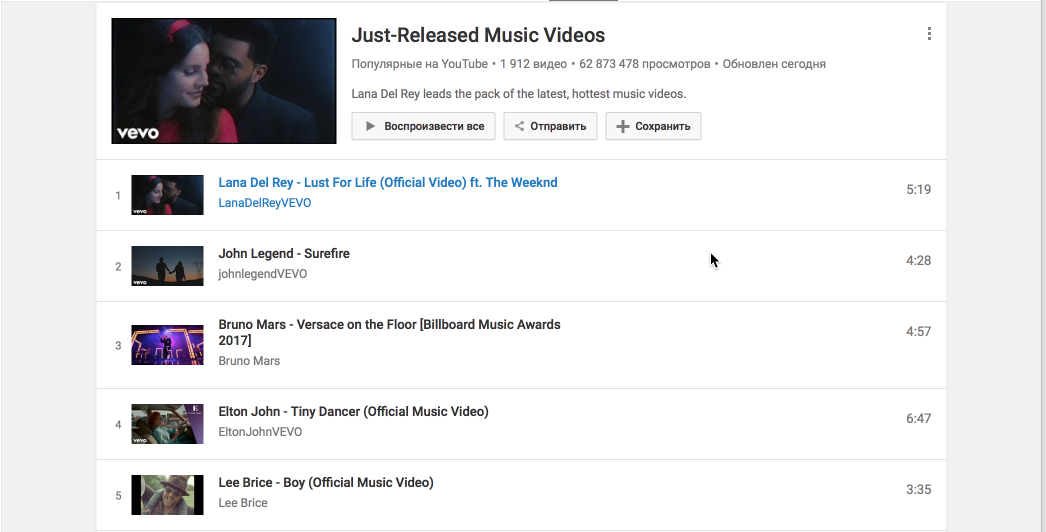
\includegraphics[scale=0.4]{youtubejustreleased.png}
  \caption{ Изображение сервиса YouTube Just Released Music Videos }
  \label{fig:domain:youtube_just_released_music_videos:picture}
\end{figure}

\subsubsection{AllMusic}
\label{sub:domain:analogues_review:allmusic}
~\newline
\indent AllMusic представляет собой американский сервис, который включает в себя крупную онлайновую музыкальную базу данных. В AllMusic представлена информация о жанрах музыки, музыкантах и коллективах, в том числе новые публикации и профессиональные рецензии. Данный сервис является обладателем огромного музыкального архива, который насчитывает около шести миллионов композиций. Также на сайте имеется возможность оценки публикаций пользователями.
AllMusic предоставляет пользователю довольно широкий спектр возможностей. Например, пользователь может подписаться на обновления, чтобы получать письма с уведомлением о новой публикации. Также есть возможность получать индивидуальные музыкальные рекомендации. Для этого необходимо заполнить артистов, которые нравятся пользователю, в поля для ввода и далее будут предложены альбомы артистов по каким-либо параметрам схожих с введенными ранее. Я считаю, что это весьма полезная функциональность для того, чтобы найти новую музыку.
AllMusic обладает стильным, выдержанным, но, на мой взгляд, слегка загроможденным дизайном. Сервис предоставляет широкую функциональность, и по этой причине пользователю, заинтересованному лишь в получении музыкальных новинок, может мешать наличие множества разнообразных разделов. Сервис перестает быть сконцентрированным на одной вещи. Это, в зависимости от интересов конечного пользователя, может как оттолкнуть, так и быть интересным.
\clearpage

\begin{figure}[ht]
\centering
  
\includegraphics[scale=0.4]{allmusic.png}
  \caption{ Изображение сервиса AllMusic }
  \label{fig:domain:allmusic:picture}
\end{figure}

Преимущества AllMusic:

\begin{itemize}
  \item возможность регистрации через социальные сети;
  \item большая база данных публикаций;
  \item возможность оценивать альбомы, что позволяет пользователям судить о качестве;
  \item богатство жанров;
  \item возможность получать уведомления;
  \item наличие персональных рекомендаций;
  \item возможность прослушать отрывки композиций.
\end{itemize}

Также можно обозначить следующие недостатки:

\begin{itemize}
  \item отсутствие концентрированности на публикациях артистов, и, как следствие, массивный интерфейс;
  \item отсутствие ссылок на сервисы для приобретения альбомов;
  \item отсутствие возможности импортировать артистов с устройств/сервисов;
  \item небольшая интерактивность.
\end{itemize}

\subsubsection{Вывод}
~\label{sub:domain:analogues_review:conclusion}
\newline
\indent Учитывая результаты ознакомления с уже присутствующими аналогами сервисов для получения информации о новинках музыкальной индустрии, можно сделать вывод, что большинство подобных сервисов либо слишком усложнены, либо делают акцент не на основную потребность конечного пользователя, а именно получение уведомлений, информации о новых публикациях любимых артистов.

\subsection{Музыкальный альбом (публикация)}
\label{sub:domain:music_album}
Музыкальный альбом~\cite{release_doc} -- это некоторая совокупность музыкальных композиций, которые выпускаются вместе, в стандартном формате. Такие композиции должны быть доступны для произведения на популярных воспроизводящих устройствах.
Существуют классификации альбомов по нескольким признакам: по объемы, типу записи и так далее. Некоторые из них будут рассмотрены далее.

\subsubsection{Классификация по объему}
\label{sub:domain:music_album:volume_classification}
~\newline
\indent Музыкальные альбомы по объему классифицируются следующим образом:
\begin{itemize}
  \item Сингл не относят к альбомам, так как состоят из одной-двух песен. Рассматривается в данной работе для большей ясности нижеприведенной информации.
  \item Стандартный альбом, или LP (от английского “Long Play”) обычно размещается на одной пластинке или же на одном компакт-диске. Время звучания насчитывает около 30-80 минут.
  \item Мини-альбом, или EP (от английского “Extended Play”) по своему размеру является промежуточным вариантом между стандартным и синглом.
  \item Двойной альбом выпускается на двух носителях информации, и время звучания такого альбома в среднем в два раза больше, чем стандартный альбом.
\end{itemize}

\subsubsection{Классификация по типам записей и композиций}
\label{sub:domain:music_album:records_type_classification}
~\newline
\indent Музыкальные альбомы по типам записей и композиций классифицируются следующим образом:
\begin{itemize}
  \item Студийный альбом -- альбом, записанный в звукозаписывающей студии.
  \item Концертный альбом -- альбом, который записывается в то время, как идет “живое” выступление перед публикой, то есть запись концерта.
  \item “Программный” альбом -- альбом, в котором обычно содержаться только ранее не издававшиеся композиции, хотя бывают и исключения, когда в “программный” альбом включаются концертные записи.
\end{itemize}

\subsubsection{Другие типы альбомов}
\label{sub:domain:music_album:other_types_classification}
~\newline
\indent Существуют также следующие типы музыкальных публикаций:
\begin{itemize}
  \item Демо представляет собой демонстрационную запись. В ней обычно содержится “сырой” материал, который используется для ознакомления других лиц с творчеством исполнителя. Зачастую это некоторые первые записи музыкантов, которые официально не издавались.
  \item Концептуальный альбом -- это альбом, все композиции которого объединены некоторой идеей (концепцией). В таких альбомах можно усмотреть некоторый замысел в составе и порядке композиций.
  \item Промо -- альбом, который выпускается небольшим тиражом специально для бесплатного распространения с целью рекламы исполнителя.
  \item Саундтрек -- альбом, в составе которого используются композиции из одного или нескольких фильмов, компьютерных игр.
  \item Трибьют -- альбом, в котором в дань уважения и в знак почитания творчества одни исполнители переигрывают песни другого определенного исполнителя. Такие композиции называются каверами.
\end{itemize}

\subsection{API}
\label{sub:domain:api}
API(application programming interface, программный интерфейс приложения) - это совокупность процедур, функций, и классов и т.д. , которую предоставляет сервис для использования в некоторых внешних приложениях (клиентах).

API~\cite{api_doc} используется для того, чтобы представить функциональность программы, при этом абстрагируясь от конкретной реализации.

WebAPI -- это API, основу в котором составляют HTTP-запросы и HTTP-ответы, сконструированные по определенным принципам. API используется, как источник данных для клиентского приложения. Клиент использует HTTP-запросы с глаголами GET, POST, PATCH, DELETE и другие. При этом в теле запроса передаются необходимые параметры. Далее API принимает этот запрос, и, если необходимо, авторизирует клиент. Может использоваться ролевая авторизация, когда в системе присутствуют разные типы пользователей: администраторы, модераторы, конечные пользователи. После запрос обрабатывается, и возвращается ответ в виде XML или JSON. Ответ принимается клиентом, также обрабатывается и на основе результатов производятся необходимые действия.

Реализация API помогает явно разделить работу backend-разработчика и frontend-разработчика, позволяя сконцентрироваться на своих сильных сторонах и разделяя зоны ответственности.


\lstset{style=fsharpstyle}

\section{Обзор используемых технологий}
\label{sec:technologies}

\subsection{Ruby on Rails}
\label{sub:technologies:ruby_on_rails}
Ruby on Rails -- веб-фреймоворк, написанный на языке Ruby~\cite{ruby_documentation}. Ruby on Rails известен тем, что позволяет очень быстро начать разрабатывать приложения. В данном веб-фреймворке есть возможность под названием ``scaffold'', которая позволяет одной командой создавать представления, контроллер и модель для нужного объекта.

Философия Ruby on Rails складывается из двух основных пунктов:

\begin{itemize}
  \item ``Convention over configuration'' -- что переводится, как преобладание соглашений над конфигурацией. Это означает, что в экосистеме Ruby on Rails разработчикам предлагается пользоваться общепринятыми соглашениями для того, чтобы ускорить разработку. Например, названия таблиц в БД должны называться множественным числом модели, для которой создается таблица. Также в настройках самого фреймворка присутствует множество дефолтных значений. Это не означает, что разработчик не может сконфигурировать приложение по своему желанию. Такая возможность, безусловно, присутствует, однако предлагается пользоваться соглашениями. Это не только ускоряет разработку, но и увеличивает уровень взаимопонимая в команде.
  \item ``DRY'' -- что расшифровывается, как ``don't repeat yourself''. Это означает избегать дублирования кода. Желательно писать приложение таким образом, чтобы оно легко масштабировалось, методы и компоненты могли быть переиспользованы в различных местах.
\end{itemize}

В Ruby on Rails используется ORM ActiveRecord. ORM представляет собой прослойку между логической моделью и е представлением в БД. ActiveRecord предоставляет богатый функционал для работы с моделями. ActiveRecord - это также шаблон проектирования. Принцип работы ActiveRecord состоит в том, что в приложении создается класс, который отображается на таблицу в БД, так что:

\begin{itemize}
  \item любой объект класса, унаследованного от ActiveRecord::Base отображается на строку в таблице БД;
  \item чтобы создать новую запись в таблице, нужно создать новый валидный объект;
  \item в качестве свойств объекта выступают поля в соответствующей строке БД;
  \item строка в таблице БД изменяется или удаляется, если изменяется или удаляется объект ActiveRecord::Base.
\end{itemize}

Также ActiveRecord предоставляет инструмент манипулирования таблицами посредством миграций - методов, в которых на языке Ruby описываются действия с БД. Для создания столбцов таблиц ActiveRecord предлагает следующие типы:

\begin{itemize}
  \item binary;
  \item boolean;
  \item date;
  \item datetime;
  \item decimal;
  \item float;
  \item integer;
  \item bigint;
  \item primary\_key;
  \item references;
  \item string;
  \item text;
  \item time;
  \item timestamp.
\end{itemize}

Веб-фреймворки в большинстве своем обладают HTML-процессорами, которые позволяют дополнять HTML-разметку различными вставками, и Ruby on Rails не является исключением. Стандартный HTML-процессор в Ruby on Rails называется ERB~\cite{erb_doc}. Он позволяет помещать в HTML-разметку Ruby-код, который создается в контроллере, тем самым давая возможность разработчикам избежать статических HTML-страниц. Однако помимо ERB существуют и другие HTML-процессоры, которые предоставляют возможность не только дополнять HTML-разметку, но и вводить новый вид разметки веб-страниц со вставками Ruby-кода.

В Ruby on Rails присутствует инструмент для соответствия URL-адреса определенному методу в контроллере. Такой инструмент называется router или маршрутизатор. В проекте, созданном на базе Ruby on Rails, существует файл routes.rb, в который помещаются так называемые маршруты. В маршрутизаторе есть возможность не только создавать маршруты не только по одному, но и целыми группами с помощью методы resources, который предлагает создание всех необходимый операций для ресурса: CREATE, READ, UPDATE, DELETE -- посредством HTTP запросов.

Выбор фреймворка Ruby on Rails для разработки обусловлен удобством его использования, расширяемостью его с помощью различных библиотек, созданных Ruby on Rails-сообществом, которое на протяжении не менее десяти лет активно развивается и предлагает богатый выбор инструментов для разработки.

\subsection{AngularJS}
\label{sub:technologies:angular_js}
AngularJS -- javascript-фреймворк, созданный в компании Google, совершивший прорыв в веб-разработке. AngularJS позволяет создавать динамические SPA. AngularJS, как и Ruby on Rails, обладает MVC-архитектурой. На момент создания AngularJS эта архитектура была революционной по причине того, что javascript-код преимущественно представлял отдельные неорганизованные скрипты, которые очень сложно масштабировать. Данный фреймворк в свою очередь предлагает разделить код на контроллеры, представления и модели(ресурсы), которые в свою очередь могут находиться в отдельных модулях.

AngularJS взаимодействует с HTML, который содержит пользовательские атрибуты, описывающиеся директивами, и соединяет переменные ввода и вывода с помощью объекта JavaScript, значения которых либо задаются вручную, либо извлекаются из некоторых JSON-данных.

AngularJS придерживается философии о том, что для проектирования пользовательских интерфейсов лучше всего подходит декларативное программирование, а для построения бизнес-логики больше подходит императивное программирование.

Фреймворк AngularJS предлагает расширение обыкновенного HTML для обеспечения двусторонней привязки данных, которая позволяет синхронизировать модели (объекты, связанные с бизнес-логикой) и HTML-код. Он упрощает тестирование и позволяет меньше работать с DOM-объектами.

Цели разработки на AngularJS:

\begin{itemize}
  \item отделение логики приложения от манипуляций с DOM-деревом;
  \item поощрение тестирования;
  \item отделение серверной стороны приложения от клиентской, что позволяет разрабатывать эти стороны параллельно.
\end{itemize}

Также AngularJS использует такой паттерн как "внедрение зависимостей", который упрощает использование компонентов приложения тем, что нет необходимости каждый раз создавать объекты классов. Внедряя компонент, система сама заботится о том, чтобы был создан объект нужного класса.

Описывая директивы AngularJS, можно сказать, что они позволяют давать HTML-тегам некоторое поведение. Директивы бывают пользовательские и встроенные. Опишем вкратце некоторые встроенные директивы:

\begin{itemize}
  \item ng-app - делает элемент, к которому применен, корневым для этого приложения;
  \item ng-class - позволяет динамически добавлять классы к элементам в HTML коде;
  \item ng-show/ng-hide - позволяет показывать/скрывать элемент на основе результата логического выражения;
  \item ng-if - добавляет или удаляет элемент из DOM-дерева на основе результата логического выражения;
  \item ng-bind - заменяет текст, содержащийся в элементе, на результат переданного выражения;
  \item ng-model - позволяет обеспечить двустороннее связывание данных;
  \item ng-repeat - аналог foreach, позволяющий проитерироваться по коллекции и создать DOM-элемент для каждого элемента в коллекции.
\end{itemize}

AngularJS выбран по причине удобства использования, скорости работы в сравнении с такими библиотеками, как jQuery, в которых отсутствует компонентный подход, MVC-архитектура и т.д.

\subsection{Bootstrap}
\label{sub:technologies:bootstrap}
Bootstrap - это CSS-фреймворк, который помогает разрабатывать фронтенд приложения.

До создания этого фреймворка разработчикам приходилось писать CSS-код, самим придумывая некоторую структурированность. Но с приходом данного фреймворка разработчики могут использовать встроенные значки, которые называются glyphicons, сетку элементов, размещая HTML-элементы без использования табличной верски и свойств типа margin, align и т.д., встроенные классы для придания элементам красивого вида и многие другие возможности.

Одним из главных преимуществ Bootstrap является сетка расположения элементов. Она работает таким образом, что элементы распологаются в таблице, строка за строкой. Строки обозначаются классом ``row'', и каждая строка разделяется на 12 столбцов, которые могут быть объединены. Для обозначения необходимого колчества столбцов нужно элементу div написать класс ``col-y-x'', где y - это предполагаемый размер экрана и принимающий значения ``sm'', ``md'', ``lg'', а x - это количество необходимых ячеек от 1 до 12.


\section{Проектирование и реализация} % (fold)
\label{sec:arch_and_realization}


Разработанное программное обеспечение представляет из себя приложение, написанное на фреймворке \ror.
Приложение предназначено для получения новинок музыкальной индустрии или, другими словами, музыкальных релизов выбранных пользователем музыкантов.

\subsection{Проектирование приложения}
\label{sub:arch_and_mod:design}
При проектировании приложения обязательно следует учитывать фактор изменяемости и заложить возможности расширяемости. Учитывая эти факторы, можно приступать к написанию приложения с осознанием того факта, что в будущем не придётся переписывать его полностью с нуля. Всё, что будет нужно - это добавить новые компоненты, то есть расширить систему.

В случае сервиса, предоставляющего возможность получения новинок музыкальной индустрии, расшираяемость будет выражаться в том, чтобы была возможность добавить новые сторонние сервисы, которые предоставляют свой API для использования ресурсов.

Проектирование БД в данной работе можно начать с модели пользователя. Пользователь - одна из ключевых фигур в работе сервиса. Пользователю должны быть доступны:

\begin{itemize}
  \item регистрация;
  \item аутентификация;
  \item авторизация;
  \item доступ к непосредственным возможностям сервиса.
\end{itemize}

Для упрощения реализации вышеуказанных возможностей в сервисе используется библиотека Devise. Она диктует создание модели пользователя определённым образом, чтобы можно было легко использовать встроенные в неё инструменты: регистрация, аутентификация, восстановление пароля, подтверждение регистрации и др. Таким образом, модель пользователя будет состоять из следующих полей:

\begin{itemize}
  \item id;
  \item email;
  \item encrypted\_password;
  \item reset\_password\_token;
  \item confirmation\_token;
  \item created\_at;
  \item updated\_at.
\end{itemize}

В действительной таблице пользователя полей несколько больше, но этого объёма достаточно, чтобы передать основные направления проектирования модели пользователя.

Далее рассмотрим модель артиста. Учитывая тот факт, что в сервисе будут использоваться сторонние приложения и их API, нужно отметить, что у каждого из них своё строение. В данной версии сервиса будет использоваться три сторонних приложения, информация двух из которых будет по мере использования сервиса сохраняться в БД. Эти два сервиса: Discogs и RateYourMusic. В каждом из этих сервисов есть информация об артистах. Поэтому было принято решение создать две модели: DiscogsArtistsInfo (модель, которая отвечает за сохранение информации из веб-приложения Discogs) и RymArtistsInfo (отвечает за сохранение информации из веб-приложения, которое называется RateYourMusic).

Модель DiscogsArtistsInfo, учитывая структуру информации в приложении Discogs, включает в себя следующие поля:

\begin{itemize}
  \item id;
  \item image\_url;
  \item created\_at;
  \item updated\_at.
\end{itemize}

Учитывая структуру информации в приложении RateYourMusic, модель RymArtistsInfo включает в себя следующие поля:

\begin{itemize}
  \item id;
  \item formed\_year;
  \item disbanded\_year;
  \item genres;
  \item created\_at;
  \item updated\_at.
\end{itemize}

Также в сервисе присутствует модель, которая выступает как модель артиста уже внутри системы. Она будет соединяться с вышеописанными моделями артиста через промежуточную модель, которая будет описана позже. Таким образом, модель ArtistIdentity включает в себя следующие поля:

\begin{itemize}
  \item id;
  \item name;
  \item created\_at;
  \item updated\_at.
\end{itemize}

Музыкальная публикация, или релиз, также является ключевым понятием в сервисе. Так как работа происходит с двумя сторонними приложениями, для хранения информации о музыкальных публикациях происходит через две модели: DiscogsReleasesInfo (отвечает за сохранение информации из сервиса Discogs) и RymReleasesInfo (отвечает за сохранение информации из сервиса RateYourMusic).

DiscogsReleasesInfo содержит следующие поля:

\begin{itemize}
  \item id;
  \item format\_type;
  \item track\_list;
  \item genres;
  \item label;
  \item style;
  \item created\_at;
  \item updated\_at.
\end{itemize}

RymReleasesInfo содержит следующие поля:

\begin{itemize}
  \item id;
  \item format\_type;
  \item track\_list;
  \item genres;
  \item descriptors;
  \item created\_at;
  \item updated\_at.
\end{itemize}

Поле, обозначаемое как format\_type, несёт в себя информацию о типе релиза: сингл, extended\_play и др. Поле descriptors содержит в себе дополнительную информацию, которая может говорить об релизе и по которой потом можно проще производить поиск.

Однако так же, как и с организацией хранения артистов, необходимо иметь модель музыкальной публикации внутри системы. Такой моделью является ReleaseIdentity и включает в себя следующие поля:

\begin{itemize}
  \item id;
  \item year\_released;
  \item format\_type;
  \item created\_at;
  \item updated\_at.
\end{itemize}

Чтобы система была расширяема, необходимо сделать возможность добавления различных компонентов. В сервисе, предоставляющем возможность получения новинок музыкальной индустрии, такими компонентами являются сторонние сервисы, предоставляющие доступ к своему API. В данной реализации, как уже было сказано, используются два таких сервиса: Discogs и RateYourMusic. Для обоих сервисов в системе созданы модели как артистов, так и музыкальных публикаций (релизов). Также созданы представления артистов и релизов в самой системе в виде моделей. Для пользователя нет нужды, и даже может быть затруднительно, представлять артистов и релизы в контексте различных сторонних сервисов. Для пользователя удобнее видеть не две или более различных музыкальных публикаций, которые на самом деле являются одной и той же, но и разных сервисов, а видеть одну публикацию, информация о которой расширена и дополнена данными из сторонних API. Таким образом удается не просто избегать дублирования, но и обогащать данные. Со временем можно добавить и больше различных сторонних сервисов. Таким образом, в системе присутствует модель ArtistIdentity, которая дополняется моделями DiscogsArtistsInfo и RymArtistsInfo. Также для обозначения релизов в системе присутствует модель ReleaseIdentity, которая дополняется моделями DiscogsReleaseInfo и RymReleaseInfo. Чтобы связать эти модели, необходимо создать модель Identity, которая будет ссылаться на объекты вышеописанных моделей и включать следующие поля:

\begin{itemize}
  \item id;
  \item entity\_id;
  \item service\_entity\_id;
  \item info\_id;
  \item service\_type;
  \item entity\_type;
  \item created\_at;
  \item updated\_at.
\end{itemize}

Данная модель является надстройкой над вышеописанными моделями и связывает их определённым образом. Поле service\_type содержит имя сервиса, информацию которого содержит. В данной реализации этими именами могут быть "rym" и "discogs". В качестве значений поля entity\_type могут выступать "artist" и "release". На основе entity\_type и service\_type можно info\_id будет ссылаться на нужный объект информации релиза или артиста из того или иного сервиса.

Таким образом, опираясь на вышеописанную структуру данных в сервисе, можно строить приложение, наполняя его бизнес-логикой.

Существует множество подходов для построения архитектуры приложений. В данной дипломной работе была выбрана трёхуровневая архитектура.

\subsection{Трёхуровневая архитекутра приложения}
\label{sub:arch_and_mod:mvc}

Архитектура приложения - это определённый подход в определении взаимоотношений компонентов приложения. Обычно архитектура приложений соответствует задачам разработки. В данной дипломной работе выбрана трёхуровневая архитектура. Эти уровни называются: уровень модели, уровень контроллера и уровень представления. Иначе говоря, MVC - Model, View, Controller.

Данная архитектура используется во множестве веб-фреймворков. Она удобна тем, что позволяет разделить зоны ответственности между компонентами, облегчить тестирование, придать гибкость разработке. Фреймворк \ror{} и \ajs{} также в своей основе используют данную архитектуру.

\subsubsection{Уровень модели}
\label{sub:arch_and_mod:mvc:model}
~\newline
\indent Уровень модели -- один из трёх уровней в MVC-архитектуре. Его обязанности можно разделить на две категории:

\begin{itemize}
  \item бизнес-логика приложения;
  \item управление связью в базой данных.
\end{itemize}

Бизнес-логика включает в себя определённые правила, отношения и принципы, которые должны существовать в приложении. Эти правила могут быть выражены как в коде самого приложения, так и базе данных. Однако в данной дипломной работе бизнес-логика содержится именно в коде приложения, а именно в ruby-классах, наследующихся от класса ActiveRecord::Base, который является стандартом де-факто для моделей, использующихся во фреймворке \ror{}.

В данной дипломной работе присутствует класс ReleaseIdentity, который используется для хранения и обработки объектов музыкальных публикаций. Пример реализации класса ReleaseIdentity представлен на листинге~\ref{lst:arch_and_mod:mvc:model:release_identity_class_definition}:
\begin{lstlisting}[style=fsharpstyle,caption={Базовая реализация класса ReleaseIdentity}, label=lst:arch_and_mod:mvc:model:release_identity_class_definition]
class ReleaseIdentity < ActiveRecord::Base
end
\end{lstlisting}

Классы-наследники класса ActiveRecord::Base обладают богатым функционалом. Они содержат в себе возможности валидирования, организации связей между объектами, возможностями создания транзакций, сложных запросов в БД и многими другими. Подробнее об этом будет написано несколько позже, когда будет рассматриваться взаимодействие с БД.

Ярким примером бизнес-логики может служить проверка корректности конструируемых объектов. Например, название артиста не должно быть пустым и содержать только текстовые данные. Или же год начала карьеры артиста не может быть отрицательными или больше нынешнего года по значению. Всё это реализуется в \ror{} с помощью механизма валидации.

В данной дипломной работе присутствует класс RymArtistsInfo, который используется для хранения результатов работы с сервисом Rate Your Music\footnote{\url{https://rateyourmusic.com/}}. В этом классе присутствуют следующие поля:

\begin{itemize}
  \item id -- уникальный идентификатор записи в таблице;
  \item formed\_year -- год формирования музыкальной группы(исполнителя);
  \item disbanded\_yead -- год окончания деятельности музыкальной группы(исполнителя);
  \item genres -- жанры, которые присущи музыкальной группе(исполнителю);
  \item created\_at -- дата создания записи в БД приложения;
  \item updated\_at -- дата обновления записи в БД приложения.
\end{itemize}

В данном случае годы формирования и окончания деятельности музыкальной группы исполнителя должны придерживаться правил, описанных выше. Также строка, содержащая жанры, не может иметь длину, менее 2 символов. Для обеспечения этой части бизнес-логики я воспользовался инструментарием фреймворка \ror{}. Используя метод validates, можно добиться проверки определённых правил перед сохранением записи, чтобы хранить в базе только корректные записи. Также существует метод validate, в который передаётся название метода, в котором можно описать более сложную логику. Таким образом можно проверить то, что год окончания деятельности музыкальной группы больше или равен году начала карьеры. Пример использования продемонтрирован на листинге ~\ref{lst:arch_and_mod:mvc:model:rym_artists_info_validations}:

\begin{lstlisting}[style=fsharpstyle,caption={Реализация валидации в классе RymArtistsInfo}, label=lst:arch_and_mod:mvc:model:rym_artists_info_validations]
class RymArtistsInfo < ActiveRecord::Base
  validates :formed_year
  validates :disbanded_year, numericality: {only_integer: true, greated_than: 0, less_than: DateTime.now.year}
  validates :genres, length: {minimum: 2}
  validate disbanded_more_or_eql_formed

  private

  def disbanded_more_or_equal_formed
    disbanded_year >= formed_year
  end
end
\end{lstlisting}

Фреймворк \ror{} предлагает ещё один полезный инструмент, который называется "функция обратного вызова". Такие функции существуют и на уровне базы данных, но в этом и состоит преимущество веб-фреймворка - позволять более компактно и удобно писать необходимый функционал. Функции обратного вызова работают таким образом, что в определённые моменты жизненного цикла объектов, такие, как перед сохранением, удалением или валидированием объекта, вызываются методы, в который можный поместить необходимый для этого момента код. Это ещё одно преимущество слоя модели, потому как позволяет избегать длинных цепочек вызовов методов, а воспользоваться удобным интерфейсом для обработки моментов жизненного цикла. В \ror{} такие моменты обрабатываются путём добавления методов:
\begin{itemize}
  \item before\_save;
  \item before\_create;
  \item before\_validate;
  \item around\_save;
  \item after\_save;
  \item after\_update.
\end{itemize}

Привет функции обратного вызова представлен на листинге ~\ref{lst:arch_and_mod:mvc:model:callback}:

\begin{lstlisting}[style=fsharpstyle,caption={Пример получения артистов по определённым параметрам}, label=lst:arch_and_mod:mvc:model:callback]
  class RymReleasesInfo < ActiveRecord::Base
    after_save :set_link_to_identity

    private

    def set_link_to_identity
      ReleaseIdentity.find_or_create_by(
        title: title,
        artist: artist
      )
    end
  end
\end{lstlisting}

Стоит обратить внимание на тот факт, что с ростом приложений модели включают в себя всё больше логики и становятся очень большими. Минус этого состоит в том, что происходит нарушение одного из принципов объектно-ориентированного программирования. Это принцип единственной ответственности класса. Он нарушается в тот момент, когда класс выполняет много различных функций: используется для подключения к БД, содержания бизнес-логики, создания других объектов и т.д. Однако существует способ улучшения данной архитектуры путём введения в слой модели дополнительного компонента - сервиса. Сервисы - это такие классы или модули, который содержат в себе код, который можно извлечь из модели, чтобы её не перегружать. Например, сервисы могут содержать в себе код обращения в стороннему приложению, либо расчёт цен и многое другое. Более того, код сервисов может использоваться в различных местах, тем самым обеспечивая модульность. Это помогает проще тестировать. Кроме этого, сервисы реализуют принцип инкапсуляции, то есть принцип сокрытия реализации. Имеется в виду, что коду, использующему сервис, необязательно знать, как именно реализован тот или иной метод. Если сервис отвечает за работу с поиском и передачей музыкальных публикаций, то коду, работающему с этим сервисом не важно, берёт сервис публикации с помощью API, делает запрос в БД или же эти публикации просто лежат в массиве в памяти приложения. Сам фреймворк не предполагает наличие сервисов, но никак не препятствует их созданию. Пример сервиса, выполняющего функцию доступа к одному из сторонних приложений ~\ref{lst:arch_and_mod:mvc:model:discogs_service_example}:

\begin{lstlisting}[style=fsharpstyle,caption={Пример получения артистов по определённым параметрам}, label=lst:arch_and_mod:mvc:model:discogs_service_example]
  module DiscogsDataService

    def self.find_artists_by_name(name)
      DiscogsApiWrapper.find_artists(name: name)
    end

    def self.find_release_by_title(title)
      DiscogsApiWrapper.find_release(title: title)
    end

  end
\end{lstlisting}

Также слой модели ответственнен за работу с базой данных. Большим преимуществом данного слоя вообще и конкретно в реализации ActiveRecord является то, что данная ORM имеет один интерфейс для работы с различными базами данных, будь то PostgreSQL, MySQL, SQLite или другие. Используя классы, унаследованные от ActiveRecord::Base, можно обращаться к базе данных для того, чтобы получить список артистов, релизов или пользователей с помощью языка Ruby. Например, если необходимо сделать выборку артистов, год начала деятельности которых больше какого-то определённого, при этом не выбирая все поля, а только год прекращения деятельности и дату создания записи в БД, используется код, указанный в листинге ~\ref{lst:arch_and_mod:mvc:model:select_artist_where_year}:

\begin{lstlisting}[style=fsharpstyle,caption={Пример получения артистов по определённым параметрам}, label=lst:arch_and_mod:mvc:model:select_artist_where_year]
  artists = RymArtistsInfo.select(:disbanded_year, :created_at).where('formed_year > ?', Date.new(2000, 4, 3))
\end{lstlisting}

Таким образом, классы, унаследованные от ActiveRecord::Base предоставляют удобный интерфейс, который помогает не писать чистый SQL-код. Возможности ActiveRecord::Base не ограничиваются простыми запросами. Существуют методы, которые позволяют делать сложные JOIN-запросы, избегать проблемы "N+1" и т.д.

Стоит упомянуть, что веб-фреймворк AngularJS также использует слой модели. В качестве объектов модели в AngularJS используются так называемые ресурсы. Ресурсы используются преимущественно для работы с запросами к API. Ресурсы в AngularJS предоставляют возможность использования как стандартных REST-запросов, так и создания пользовательских. Пример ресурса на AngularJS приведен в листинге ~\ref{lst:arch_and_mod:mvc:model:angular_artists_resource}:

\begin{lstlisting}[style=fsharpstyle,caption={Пример получения артистов по определённым параметрам}, label=lst:arch_and_mod:mvc:model:angular_artists_resource]
  app = angular.module('app')

  app.factory 'Artist', ['\$resource', (\$resource) ->
    \$resource('/artists/:id', { id: '@_id' }, {
      short_info: {method: 'GET', url: '/artist/:id/short_info'}
      extended_info: {method: 'GET', url: '/artists/:id/extended_info'}
      last_releases: {method: 'GET', url: '/artists/:id/last_releases'}
    })
  ]
\end{lstlisting}

\subsubsection{Уровень контроллера}
\label{sub:arch_and_mod:mvc:controller}
~\newline
\indent Уровень контроллера - это второй уровень в MVC-архитектуре, отвечающий за соединение слоя модели и слоя представления. В контроллерах принятно получать информацию через модели из базы данных и отображать некоторым образом эту информацию в представлениях. Представления могут быть как динамическими HTML-страницами, так и просто JSON-информацией.

Контроллеры присутствуют, как в \ror{}, так и в AngularJS. Контроллеры в \ror{} принимают запросы и возвращают ответ. Контроллеры в AngularJS ответственны за то, чтобы инициализировать некоторую информацию, отображать её в представлениях и потом следить за обновлениями, происходящими на странице. Рассмотрим реализации котроллеров более подробно.

Фреймворк \ror{} заточен под REST. Таким образом, при написании контроллеров приветствуется написание методов этих контроллеров в ресурсном стиле. В системе есть ресурс Artist, то есть модель артиста. Чтобы обрабатывать эту модель в ресурсном виде, необходимо создать реализацию следующих действий:

\begin{itemize}
  \item new - метод для создания нового артиста. Данный метод контроллера может возвращать либо HTML-страницу с формой и некоторыми инициализированными значениями для выбора опций, либо, если контроллер выступает в роли API, просто возвращать некоторые начальные данные для инициализации полей для выбора;
  \item create - метод, в который приходит информация из формы и который должен её обработать и создать артиста. Если при создании артиста присутствует некоторая логика, желательно вынести её в отдельный метод модели или же сервис, чтобы не нагружать контроллер лишней ответственностью;
  \item show - метод, который либо возвращает страницу с заполненной информацией об артисте, либо, если контроллер выступает в роли API, возвращать саму информацию об артисте в формате JSON;
  \item edit - метод, который выполняет похожие на метод "new" функции за тем исключением, что предназначен для редактирования, и поля или информация, возвращаемая из метода, уже содержит в себе данные созданного артиста;
  \item update - метод, который берёт на себя обязанности по обновлению артиста. По своей функциональности похож на метод "create", но не создаёт, а обновляет артиста при необходимости;
  \item destroy - метод, который удаляет артиста;
  \item index - метод, в обязанности которого входит работа со списком артистов. Возвращает HTML-страницу с заполненным списком артистов или же возвращает список артистов в JSON-формате.
\end{itemize}

Также контроллер принимает определённые параметры как часть запроса. Например, немаловажной является функциональность пагинации, то есть разделения списка артистов по страницам. Для реализации этой функциональности используется библиотека Kaminari, которая предоставляет простой интерфейс, доступный в контроллерах и HTML-код, который можно использовать в представлениях для отображения элементов управления, содержащих номера страниц и кнопок, которые способны, например, перейти на страницу вперед иди назад, а также на первую или последнюю страницу.

Стоит упомянуть, что контроллер отвечает за то, чтобы параметры, которые приходят в метод обработки ресурса, содержали только необходимые ключи. Это необходимо для того, чтобы обезопасить себя от многих атак. Для выборки параметров существует такой инструмент, как "parameters whitelist", то есть "белый лист параметров". В контроллере описывается private-метод, который указывает, какие параметры допустимы. Название этого метода обычно состоит из двух частей, первая из которых называется именем ресурса, а вторая содержит слово "params". Таким образом, в контроллере артистов этот метод будет называться "artists\_params".

Пример кода контроллера, который обрабатывает ресурс артиста представлен на листинге ~\ref{lst:arch_and_mod:mvc:controller:artists_controller_example}.

\begin{lstlisting}[style=fsharpstyle,caption={Пример получения артистов по определённым параметрам}, label=lst:arch_and_mod:mvc:controller:artists_controller_example]
  class ArtistsController < ApplicationController

    before_action :authenticate_user!

    def index
      authorize! :index, Artist
      @artists = Artist.all
                       .page(params[:page])
                       .per(params[:per])
       respond_to do |format|
        format.js
        format.html
       end
    end

    def new
      authorize! :new, Artist
      @artist = Artist.new
      respond_to do |format|
       format.js
       format.html
      end
    end

    def create
      authorize! :create, Artist
      @artist = Artist.create(artists_params)
      respond_to do |format|
        if @artist.save
          format.html { redirect_to @artist }
          format.json { render :show, status: :created}
        else
          format.html { render :new }
          format.json { render json: @artist.errors, status: :unprocessable_entity }
        end
      end
    end

    def show
      authorize! :show, Artist
      @artist = Artist.find(params[:id])
      respond_to do |format|
       format.js
       format.html
      end
    end

    def edit
      authorize! :show, Artist
      @artist = Artist.find(params[:id])
      respond_to do |format|
       format.js
       format.html
      end
    end

    def update
      authorize! :update, Artist
      @artist = Artist.find(params[:id])
      respond_to do |format|
        if @artist.save
          format.html { redirect_to @artist }
          format.json { render :show, status: :created}
        else
          format.html { render :edit }
          format.json { render json: @artist.errors, status: :unprocessable_entity }
        end
      end
    end

    def destroy
      authorize! :destroy, Artist
      @artist = Artist.find(params[:id])
      redirect_to artists_path
    end

    private

    def artists_params
      params.require(:artist).permit(:name,
                                     :formed_year,
                                     :disbanded_year,
                                     genres: [] )
    end

  end
\end{lstlisting}

Помимо непосредственных обработки запросов и возвращения ответов в обязанности контроллера входит проверять права доступа для определённых методов. Например, список артистов может просматривать и не аутентифицированный пользователь, но создать артиста может только зарегистрированный и аутентифицированный. А изменять пользователя может только пользователь с ролью администратора. В данном случае используется авторизация. То есть в некоторых случаях таких, как, например, редактирование модели артиста, для операции необходим функционал аутентификации и авторизации.

Для реализации авторизации приложения применяется библиотека, которая называется CanCanCan. Принцип работы состоит в том, что разработчики описывают так называемые политики, которые потом используются для проверки прав доступа. Пример написания политик приведён на листинге ~\ref{lst:arch_and_mod:mvc:controller:cancancan_example}.

\begin{lstlisting}[style=fsharpstyle,caption={Пример получения артистов по определённым параметрам}, label=lst:arch_and_mod:mvc:controller:cancancan_example]
  class Ability
    include CanCan::Ability

    def initialize(user)
      role == user.role
      artists_abilities(user, role)
    end

    private

    def artists_abilities(user, role)
      if role == :system_admin
        can [:index, :new, :create, :edit, :update, :show, :destroy]
      else
        can [:index, :new, :create, :show]
      end
    end

  end

\end{lstlisting}

В AngularJS контроллеры выступают в роли связующего звена между представлением и некоторой логикой. В AngularJS присутствует переменная \$scope, которой динамически присваиваются свойства и потом к ним можно получить доступ в представлениях. Так и устроен механизм. В AngularJS есть ещё одна возможность, которая позволяет автоматически отслеживать изменения некоторых полей и производить некоторые действия на основе этих изменения. Такая функция называется \$watch, она доступна в контроллерах AngularJS и принимает функцию, аргументами которой являются старое и новое значения отслеживаемого свойства \$scope-переменной. Когда переменная меняется, например, в нашем случае, в строке поиска артиста по имени, мы вводим букву, и, соответственно свойство, применённое к этому полю, меняется, то вызывается функция, переданная в \$watch. Тем временем массив предполагаемых артистов, который при инициализации контроллера является пустым, наполняется артистами, пришедшими с API по запросу, содержащему введенную в поле строку. Код контроллера поиска артиста представлен на листинге ~\ref{lst:arch_and_mod:mvc:controller:angular_controller_example}:

\begin{lstlisting}[language=JavaScript,caption={Пример получения артистов по определённым параметрам}, label=lst:arch_and_mod:mvc:controller:angular_controller_example]
  app = angular.module('app')

  app.controller 'ArtistsSearchController', ['$scope', 'Artist', ($scope, Artist) ->

  $scope.artistTitle = ''
  $scope.artists = []

  $scope.$watch('addedProductId', (newValue, oldValue) ->
    if newValue.length > 2
      Artist.search({title: newValue}, (response) ->
        $scope.artists = response.artists
      )
  )
\end{lstlisting}

\subsubsection{Уровень представления}
\label{sub:arch_and_mod:mvc:view}
~\newline
\indent Уровень представления - это третий слой MVC-архитектуры. Он отвечает отображение информации пользователю. Задача уровня представления - быть понятной и привлекательной. В данной дипломной работе уровень представления реализуется тремя библиотками: \ror{}(когда используются HTML-страницы в ответах на запросы), AngularJS(когда используются HTML-шаблоны со вставками angular-кода, управляемыми angular-контроллерами) и Bootstrap(когда необходимы стили для элементов и сетка для их размещения).

%% пример кода Ruby on Rails + Bootstrap (artists list)

Фреймворк \ror{} обладает встроенным HTML-препроцессором и позволяет помещать в HTML части ruby-кода. Оно работает таким образом, что в контроллере инициализируются некоторые переменные и потом используются в представлениях. Пример представления, содержащего список артистов, представлен на листинге ~\ref{lst:arch_and_mod:mvc:controller:rails_view_example}:

\begin{lstlisting}[language=HTML5,caption={Пример получения артистов по определённым параметрам}, label=lst:arch_and_mod:mvc:controller:rails_view_example]
  <div class="container">
    <div class="row">
      <div class="col-md-12">
        <%= @artists.each do |artist|%>
          <h2>Title</h2>
          <h3> <%= artist.title %> </h3>
          <div class="image-container">
            <%= artist.main_image_path %>
          </div>
          <%= link_to 'Show details', artists_path(artist), class: 'btn btn-info' %>
        <% end %>
      </div>
    </div>
  </div>
\end{lstlisting}
%% пример кода AngularJS + Bootstrap (search artist)

Аналогичным образом работает и AngularJS с тем отличием, что данные, которыми он пользуется в представлениях, инициализируются в контроллерах. То, как данные попадают в контроллер, уже не заботит представление. В контроллерах AngularJS присутствует переменная \$scope, которая, как клей, связывает контроллер и представление. Пример представления для поиска артиста представлен на листинге ~\ref{lst:arch_and_mod:mvc:controller:angular_view_example}:

\begin{lstlisting}[language=HTML5,caption={Пример получения артистов по определённым параметрам}, label=lst:arch_and_mod:mvc:controller:angular_view_example]
  <div class="container">
    <div class="row">
      <div class="col-md-12">
        <input name="artist-search" ng-model="searchTitle" class="form-control"/>
        <div ng-show="searchResults">
          <ul class="item-list">
            <li class="item" ng-repeat="result in searchResults">
              <span>{{result.title}}</span>
              <img src="{{result.image_src}}" />
            </li>
          </ul>
        </div>
      </div>
    </div>
  </div>
\end{lstlisting}


\subsubsection{Написание программного кода для работы с сторонними API}
\label{sub:arch_and_mod:mvc:controller}
~\newline
\indent Сервис, предоставляющий возможность получения новинок музыкальной индустрии основан на том, что получает информации из сторонних источников. В качестве таких источников выступают веб-сервисы. Одни из них предоставляют программный интерфейс, с помощью которого можно обращаться к сервису, составляя запросы с определёнными параметрами и получая ответы. Другие же не предоставляют такой интерфейс, и, если необходима информация из такого источника, то необходимо с помощью определённых инструментов таких, как Nokogiri, парсить страницы этих сервисов по алгоритмам, которые предусматривают в некоторых случаях автоматическое заполнение, например, строки поиска, размещённой на странице такого сервиса, ожидание ответа, перенаправления на страницу с результатами поиска. После этого необходимо открывать все ссылки и разбирать страницу по элементам. Если же в сервисе нет строки поиска или элемента управления, используя который можно найти необходимую информацию, то можно пойти способом перебора ссылок на страницы с нужной информацией путём изменения id или slug необходимых ресурсов. Такой способ имеет ряд недостатков:

\begin{itemize}
  \item привязанность к структуре веб-страниц;
  \item получение информации не напрямую из БД, а из представлений;
  \item необходимость учёта большого количества факторов для успешного парсинга;
  \item небольшая польза тестирования из-за непостоянной структуры данных;
  \item необходимость переписания кодовой базы при изменении содержимого страниц стороннего сервиса.
\end{itemize}

Вторым видом получения информации из стороннего приложения является использование API. Разработчики сервиса предоставляют интерфейс для доступа путём создания запросов на сервер приложения. Этот способ очень удобен, так как позволяет получать именно необходимую информацию заранее спланированным способом.

Для использования этого методы необходимо реализовать так называемую "обертку". Используя некоторый инструмент, способный делать запросы на удалённый сервер, пишутся методы, которые внутри себя используют обращения к API. Тем самым соблюдается принцип инкапсуляции, когда программист, использующий впоследствии эти методы, не заботится о том, из какого источника берутся данные. Преимущества данного метода:

\begin{itemize}
  \item получение необходимого количества информации за запрос;
  \item определённая структура обращений;
  \item возможность тестирования, которое будет полезным;
  \item малое время интеграции и написание кодовой базы.
\end{itemize}

Написать "обертку" для API можно несколькими способами. Первый способ -- это написание так называемого гема. Так называются библиотеки в Ruby, которые потом загружаются в общее хранилище и могут быть использованы другими разработчиками. А второй способ - это написание модуля в кодовой базе приложения. Плюсы гема состоят в том, что разработчик оказывает пользу сообществу, внося свой вклад, но тем самым возлагая на себя ответственность за качество гема. В этом и заключаются минусы гема - необходимо тестирование. Когда пишешь небольшой модуль в приложении, можно себе довериться и не тратить время на тестирование.

При написании "обёртки для API" также важно учесть такое понятие, как "throttling". Оно означет то, что есть ограничение запросов к API в секунду. При превышении данного лимита могут быть последствия в виде блокировок. Необходимо использовать некоторые инструменты, которые будут ограничивать количество запросов.

Пример "обертки" для сервиса Discogs представлен на листинге ~\ref{lst:arch_and_mod:mvc:controller:discogs_wrapper_example}:


\begin{lstlisting}[style=fsharpstyle,caption={Пример получения артистов по определённым параметрам}, label=lst:arch_and_mod:mvc:controller:discogs_wrapper_example]
  require 'httparty'
  require 'api_cache'
  require 'awesome_print'

  class DiscogsApiWrapper

    include HTTParty

    debug_output $stdout

    attr_accessor :token

    HEADERS = {
      'User-Agent' => 'BrigntSoundApi/0.0.0'
    }

    API_CACHE_OPTIONS = {
      :cache => 3600,
      :valid => :forever,
      :period => 2,
      :timeout => 5,
      :fail => -1
    }

    base_uri 'https://api.discogs.com/'

    format :json

    def initialize(opts = {})
      @token = opts[:token]
    end

    def get_releases(artist_id, page = 1, per_page = 10)
      query = encoded_query({
        page: page,
        per_page: per_page,
        token: token
      })
      self.class.get(
        "/artists/#{artist_id}/releases",
        headers: HEADERS,
        query: query,
        debug_output: $stdout
      )
    end

    def search_for_artist(artist_name = '', page = 1, per_page = 10)
      query = encoded_query({
        type: 'artist',
        q: artist_name,
        page: page,
        per_page: per_page,
        token: token
      })
      APICache.get("artist", API_CACHE_OPTIONS) do
        self.class.get(
          "/database/search",
          headers: HEADERS,
          query: query
        )
      end
    end

    private

    def encoded_query(params)
      URI.encode_www_form(params)
    end
  end

\end{lstlisting}


\newcommand{\byr}{Br}

\section{Технико-экономическое обоснование эффективности сервиса, предоставляющего возможность получения новинок музыкальной индустрии}

% Begin Calculations

\FPeval{\totalProgramSize}{8980}
\FPeval{\totalProgramSizeCorrected}{8400}

\FPeval{\normativeManDays}{224}

\FPeval{\additionalComplexity}{0.08}
\FPeval{\complexityFactor}{clip(1 + \additionalComplexity)}

\FPeval{\stdModuleUsageFactor}{0.7}
\FPeval{\originalityFactor}{0.9}

\FPeval{\adjustedManDaysExact}{clip( \normativeManDays * \complexityFactor * \stdModuleUsageFactor * \originalityFactor )}
\FPround{\adjustedManDays}{\adjustedManDaysExact}{0}

\FPeval{\daysInYear}{365}
\FPeval{\redLettersDaysInYear}{9}
\FPeval{\weekendDaysInYear}{104}
\FPeval{\vocationDaysInYear}{21}
\FPeval{\workingDaysInYear}{ clip( \daysInYear - \redLettersDaysInYear - \weekendDaysInYear - \vocationDaysInYear ) }

\FPeval{\developmentTimeMonths}{4}
\FPeval{\developmentTimeYears}{0.25}
\FPeval{\developmentTimeYearsExact}{clip(\developmentTimeMonths / 12)}
\FPround{\developmentTimeYears}{\developmentTimeYearsExact}{2}
\FPeval{\requiredNumberOfProgrammersExact}{ clip( \adjustedManDays / (\developmentTimeYears * \workingDaysInYear) + 0.5 ) }

% тут должно получаться 2 ))
\FPtrunc{\requiredNumberOfProgrammers}{\requiredNumberOfProgrammersExact}{0}

\FPeval{\tariffRateFirst}{250}
\FPeval{\tariffFactorFst}{3.04}
\FPeval{\tariffFactorSnd}{3.48}


\FPeval{\employmentFstExact}{clip( \adjustedManDays / \requiredNumberOfProgrammers )}
\FPtrunc{\employmentFst}{\employmentFstExact}{0}

\FPeval{\employmentSnd}{clip(\adjustedManDays - \employmentFst)}


\FPeval{\workingHoursInMonth}{160}
\FPeval{\salaryPerHourFstExact}{clip( \tariffRateFirst * \tariffFactorFst / \workingHoursInMonth )}
\FPeval{\salaryPerHourSndExact}{clip( \tariffRateFirst * \tariffFactorSnd / \workingHoursInMonth )}
\FPround{\salaryPerHourFst}{\salaryPerHourFstExact}{0}
\FPround{\salaryPerHourSnd}{\salaryPerHourSndExact}{0}

\FPeval{\bonusRate}{1.5}
\FPeval{\workingHoursInDay}{8}
\FPeval{\totalSalaryExact}{clip( \workingHoursInDay * \bonusRate * ( \salaryPerHourFst * \employmentFst + \salaryPerHourSnd * \employmentSnd ) )}
\FPround{\totalSalary}{\totalSalaryExact}{0}

\FPeval{\additionalSalaryNormative}{20}

\FPeval{\additionalSalaryExact}{clip( \totalSalary * \additionalSalaryNormative / 100 )}
\FPround{\additionalSalary}{\additionalSalaryExact}{0}

\FPeval{\socialNeedsNormative}{0.6}
\FPeval{\socialProtectionNormative}{34}
\FPeval{\socialProtectionFund}{ clip(\socialNeedsNormative + \socialProtectionNormative) }

\FPeval{\socialProtectionCostExact}{clip( (\totalSalary + \additionalSalary) * \socialProtectionFund / 100 )}
\FPround{\socialProtectionCost}{\socialProtectionCostExact}{0}

\FPeval{\taxWorkProtNormative}{4}
\FPeval{\taxWorkProtCostExact}{clip( (\totalSalary + \additionalSalary) * \taxWorkProtNormative / 100 )}
\FPround{\taxWorkProtCost}{\taxWorkProtCostExact}{0}
\FPeval{\taxWorkProtCost}{0} % это считать не нужно, зануляем чтобы не менять формулы

\FPeval{\stuffNormative}{3}
\FPeval{\stuffCostExact}{clip( \totalSalary * \stuffNormative / 100 )}
\FPeval{\stuffCost}{\stuffCostExact}

\FPeval{\timeToDebugCodeNormative}{15}
\FPeval{\reducingTimeToDebugFactor}{0.3}
\FPeval{\adjustedTimeToDebugCodeNormative}{ clip( \timeToDebugCodeNormative * \reducingTimeToDebugFactor ) }

\FPeval{\oneHourMachineTimeCost}{5000}

\FPeval{\machineTimeCostExact}{ clip( \oneHourMachineTimeCost * \totalProgramSizeCorrected / 100 * \adjustedTimeToDebugCodeNormative ) }
\FPround{\machineTimeCost}{\machineTimeCostExact}{0}

\FPeval{\businessTripNormative}{7}
\FPeval{\businessTripCostExact}{ clip( \totalSalary * \businessTripNormative / 100 ) }
\FPround{\businessTripCost}{\businessTripCostExact}{0}

\FPeval{\otherCostNormative}{10}
\FPeval{\otherCostExact}{clip( \totalSalary * \otherCostNormative / 100 )}
\FPround{\otherCost}{\otherCostExact}{0}

\FPeval{\overheadCostNormative}{8}
\FPeval{\overallCostExact}{clip( \totalSalary * \overheadCostNormative / 100 )}
\FPround{\overheadCost}{\overallCostExact}{0}

\FPeval{\overallCost}{clip( \totalSalary + \additionalSalary + \socialProtectionCost + \taxWorkProtCost + \stuffCost + \machineTimeCost + \businessTripCost + \otherCost + \overheadCost ) }

\FPeval{\supportNormative}{30}
\FPeval{\softwareSupportCostExact}{clip( \overallCost * \supportNormative / 100 )}
\FPround{\softwareSupportCost}{\softwareSupportCostExact}{0}


\FPeval{\baseCost}{ clip( \overallCost + \softwareSupportCost ) }

\FPeval{\profitability}{35}
\FPeval{\incomeExact}{clip( \baseCost / 100 * \profitability )}
\FPround{\income}{\incomeExact}{0}

\FPeval{\estimatedPrice}{clip( \income + \baseCost )}

\FPeval{\localRepubTaxNormative}{3.9}
\FPeval{\localRepubTaxExact}{clip( \estimatedPrice * \localRepubTaxNormative / (100 - \localRepubTaxNormative) )}
\FPround{\localRepubTax}{\localRepubTaxExact}{0}
\FPeval{\localRepubTax}{0}

\FPeval{\ndsNormative}{20}
\FPeval{\ndsExact}{clip( (\estimatedPrice + \localRepubTax) / 100 * \ndsNormative )}
\FPround{\nds}{\ndsExact}{0}


\FPeval{\sellingPrice}{clip( \estimatedPrice + \localRepubTax + \nds )}

\FPeval{\taxForIncome}{18}
\FPeval{\incomeWithTaxes}{clip(\income * (1 - \taxForIncome / 100))}
\FPround\incomeWithTaxes{\incomeWithTaxes}{0}

% End Calculations

\subsection{Введение и исходные данные}

Целью данной дипломной работы является создание программного продукта, позволяющего пользователю получать новинки музыкальной индустрии в виде уведомлений о недавно вышедших публикациях выбранных им музыкальных исполнителей. Данный программный продукт позволит получать информацию из нескольких источников, тем самым помогая пользователю удобнее ориентироваться среди различных сервисов, получать только необходимую и интересную информацию. Это очень эффективно, поскольку сокращается время на поиски новых публикаций самостоятельно. В экономическом смысле - это сократит расходы на подписки на несколько сервисов, которые занимаются размещением на своей платформе новых музыкальных публикаций.

Для разработчика экономическая эффективность будет определяться как прибыль от реализации, а для пользователя - как экономия затрат. Для определения экономической эффективности рассчитаем смету затрат и цену программного продукта.

\subsection{Расчёт сметы затрат и цены программного продукта}

Для представления программного продукта на рынке он должен быть законченным, иметь презентабельный вид. Для реализации программного продукта необходимо пройти через два этапа: этап, связанный с разработкой ПО(выяснение требований, программирование, тестирование, отладка), и этап, связанный с непосредственной реализацией продукта на рынке (реализация, поддержка).

Программный комплекс относится ко 2-й группе сложности. Категория новизны – “В”. Расчеты выполнены на основе методического пособия [1].

Исходные данные для проекта указаны в таблице~\ref{table:econ:initial_data}.

\begin{table}[!ht]
\caption{Исходные данные}
\label{table:econ:initial_data}
  \centering
  \begin{tabular}{| >{\raggedright}m{0.62\textwidth}
                  | >{\centering\arraybackslash}m{0.05\textwidth}
                  | >{\centering}m{0.17\textwidth}
                  | >{\centering\arraybackslash}m{0.08\textwidth}|}
    \hline
    {\begin{center}
      Наименование показателей
    \end{center} } & Буквенные обозначения & Единицы измерения & Количество \\
    \hline
    Коэффициент новизны & $ \text{К}_\text{н} $ & единиц & \num{\originalityFactor} \\
    \hline
    Группа сложности & & единиц & 2 \\
    \hline
    Дополнительный коэффициент сложности & $ \text{К}_\text{сл} $ & единиц & \num{\complexityFactor} \\
    \hline
    Поправочный коэффициент, учитывающий использование типовых программ & $ \text{К}_\text{т} $ & единиц & \num{\stdModuleUsageFactor} \\
    \hline
    Установленная плановая продолжительность разработки & $ \text{T}_\text{р} $ & лет & \num{\developmentTimeYears} \\
    \hline
    Продолжительность рабочего дня & $ \text{T}_\text{ч} $ & часов & \num{\workingHoursInDay} \\
    \hline
    Тарифная ставка 1-го разряда & $ \text{T}_\text{м1} $ & руб. & \num{\tariffRateFirst} \\
    \hline
    Коэффициент премирования & $ \text{К}_\text{п} $ & единиц & \num{\bonusRate} \\
    \hline
    Норматив дополнительной заработной платы исполнителей & $ \text{Н}_\text{д} $ & \% & \num{\additionalSalaryNormative} \\
    \hline
    Отчисления в  & $ \text{З}_\text{сз} $ & \% & \num{\socialProtectionNormative} \\
    \hline
    Отчисления в Белгосстрах & $ \text{Н}_\text{нс} $ & \% & \num{\socialNeedsNormative} \\
    \hline
    Расходы на научные командировки & $ \text{Р}_\text{нк} $ & \% & \num{\businessTripNormative} \\
    \hline
    Прочие прямые расходы & $ \text{П}_\text{з} $ & \% & \num{\otherCostNormative} \\
    \hline
    Прочие накладные расходы & $ \text{П}_\text{рн} $ & \% & \num{\overheadCostNormative} \\
    \hline
    Налог на прибыль & $ \text{П}_\text{рн} $ & \% & \num{\taxForIncome} \\
    \hline
  \end{tabular}
\end{table}

На основании сметы затрат и анализа рынка ПО определяется плановая отпускаемая цена.
Для составления сметы затрат на создание ПО необходима предварительная оценка трудоемкости ПО и его объёма.
Расчет объёма программного продукта (количества строк исходного кода) предполагает определение типа программного обеспечения, всестороннее техническое обоснование функций ПО и определение объёма каждой функций.
Согласно классификации типов программного обеспечения~\cite[с.~59,~приложение 1]{palicyn_2006}, разрабатываемое ПО с наименьшей ошибкой можно классифицировать как ПО методo"=ориентированных расчетов.


Общий объём программного продукта определяется исходя из количества и объёма функций, реализованных в программе:
\begin{equation}
  \label{eq:econ:total_program_size}
  V_{o} = \sum_{i = 1}^{n} V_{i} \text{\,,}
\end{equation}
\begin{explanation}
где & $ V_{i} $ & объём отдельной функции ПО, LoC; \\
    & $ n $ & общее число функций.
\end{explanation}

На стадии технико-экономического обоснования проекта рассчитать точный объём функций невозможно.
Вместо вычисления точного объёма функций применяются приблизительные оценки на основе данных по аналогичным проектам или по нормативам~\cite[с.~61,~приложение 2]{palicyn_2006}, которые приняты в организации.

\begin{table}[ht]
\caption{Перечень и объём функций программного модуля}
\label{table:econ:function_sizes}
\centering
  \begin{tabular}{| >{\centering}m{0.12\textwidth}
                  | >{\raggedright}m{0.40\textwidth}
                  | >{\centering}m{0.18\textwidth}
                  | >{\centering\arraybackslash}m{0.18\textwidth}|}

  \hline
         \multirow{2}{0.12\textwidth}[-0.5em]{\centering \No{} функции}
       & \multirow{2}{0.40\textwidth}[-0.55em]{\centering Наименование (содержание)}
       & \multicolumn{2}{c|}{\centering Объём функции, LoC} \tabularnewline

  \cline{3-4} &
       & { по каталогу ($ V_{i} $) }
       & { уточненный ($ V_{i}^{\text{у}} $) } \tabularnewline

  \hline
  101 & Организация ввода информации & \num{100} & \num{60} \tabularnewline

  \hline
  102 & Контроль, предварительная обработка и ввод информации & \num{520} & \num{520} \tabularnewline

  \hline
  111 & Управление вводом/выводом & \num{2700} & \num{700} \tabularnewline

  \hline
  304 & Обслуживание файлов & \num{520} & \num{580} \tabularnewline

  \hline
  305 & Обработка файлов & \num{750} & \num{750} \tabularnewline

  \hline
  309 & Формирование файла & \num{1100} & \num{1100} \tabularnewline

  \hline
  506 & Обработка ошибочных и сбойных ситуаций & \num{430} & \num{430} \tabularnewline

  \hline
  507 & Обеспечение интерфейса между компонентами & \num{730} & \num{730} \tabularnewline

  \hline
  605 & Вспомогательные и сервисные программы & \num{460} & \num{280} \tabularnewline

  \hline
  701 & Математическая статистика и прогнозирование & \num{8370} & \num{3500} \tabularnewline

  \hline

  % Уточенная оценка вычислялась с помощью R: (+ручной фикс)
  % set.seed(35)
  % locs <- c(100, 520, 2700, 520, 750, 1100, 430, 730, 460, 8370)
  % locs.which.corrected <- rbinom(length(locs), 1, 0.4)
  % locs.corrections <- rnorm(length(locs), mean = -0.25, sd=0.3)
  % locs.correction.factor <- 1 + locs.which.corrected * locs.corrections
  % locs.corrected <- signif(locs * locs.correction.factor, digits = 2)
  % locs.corrected
  % sum(locs)
  % sum(locs.corrected)

  Итог & & {\num{\totalProgramSize}} & {\num{\totalProgramSizeCorrected}} \tabularnewline

  \hline

  \end{tabular}
\end{table}

Каталог аналогов программного обеспечения предназначен для предварительной оценки объёма ПО методом структурной аналогии.
В разных организациях в зависимости от технических и организационных условий, в которых разрабатывается ПО, предварительные оценки могут корректироваться на основе экспертных оценок.
Уточненный объём ПО рассчитывается по формуле:
\begin{equation}
  \label{eq:econ:total_program_size_corrected}
  V_{\text{у}} = \sum_{i = 1}^{n} V_{i}^{\text{у}} \text{\,,}
\end{equation}
\begin{explanation}
где & $ V_{i}^{\text{y}} $ & уточненный объём отдельной функции ПО, LoC; \\
    & $ n $ & общее число функций.
\end{explanation}

Перечень и объём функций программного модуля перечислен в таблице~\ref{table:econ:function_sizes}.
По приведенным данным уточненный объём некоторых функций изменился, и общий объём ПО составил $ V_{o} = \SI{\totalProgramSize}{\text{LoC}} $, общий уточненный общем ПО~---~$ V_{\text{у}} = \SI{\totalProgramSizeCorrected}{\text{LoC}} $.

По уточненному объёму ПО и нормативам затрат труда в расчете на единицу объёма определяются нормативная и общая трудоемкость разработки ПО.
Уточненный объём ПО~---~\SI{\totalProgramSizeCorrected}{\text{LoC}}.
ПО относится ко второй категории сложности: предполагается его использование для сложных статистических расчетов и решения задач классификации, также необходимо обеспечить переносимость ПО~\cite[с.\,66, приложение~4, таблица~П.4.1]{palicyn_2006}.
По полученным данным определяется нормативная трудоемкость разработки ПО.
Согласно укрупненным нормам времени на разработку ПО в зависимости от уточненного объёма ПО и группы сложности ПО~\cite[c.~64,~приложение~3]{palicyn_2006} нормативная трудоемкость разрабатываемого проекта составляет~$ \text{Т}_\text{н} = \SI{\normativeManDays}{\text{чел.} / \text{дн.}}  $

Нормативная трудоемкость служит основой для оценки общей трудоемкости~$ \text{Т}_\text{о} $.
Используем формулу (\ref{eq:econ:effort_common}) для оценки общей трудоемкости для небольших проектов:
\begin{equation}
  \label{eq:econ:effort_common}
  \text{Т}_\text{о} = \text{Т}_\text{н} \cdot
                      \text{К}_\text{с} \cdot
                      \text{К}_\text{т} \cdot
                      \text{К}_\text{н} \text{\,,}
\end{equation}
\begin{explanation}
где & $ \text{К}_\text{с} $ & коэффициент, учитывающий сложность ПО; \\
    & $ \text{К}_\text{т} $ & поправочный коэффициент, учитывающий степень использования при разработке стандартных модулей; \\
    & $ \text{К}_\text{н} $ & коэффициент, учитывающий степень новизны ПО.
\end{explanation}

Дополнительные затраты труда на разработку ПО учитываются через коэффициент сложности, который вычисляется по формуле
\begin{equation}
\label{eq:econ:complexity_coeff}
  \text{К}_{\text{с}} = 1 + \sum_{i = 1}^n \text{К}_{i} \text{\,,}
\end{equation}
\begin{explanation}
где & $ \text{К}_{i} $ & коэффициент, соответствующий степени повышения сложности ПО за счет конкретной характеристики; \\
    & $ n $ & количество учитываемых характеристик.
\end{explanation}

Наличие двух характеристик сложности позволяет~\cite[c.~66, приложение~4, таблица~П.4.2]{palicyn_2006} вычислить коэффициент сложности
\begin{equation}
\label{eq:econ:complexity_coeff_calc}
  \text{К}_{\text{с}} = \num{1} + \num{\additionalComplexity} = \num{\complexityFactor} \text{\,.}
\end{equation}

Разрабатываемое ПО использует стандартные компоненты. Степень использования стандартных компонентов определяется коэффициентом использования стандартных модулей~---~$ \text{К}_\text{т} $.
Согласно справочным данным~\cite[c.~68,~приложение~4, таблица~П.4.5]{palicyn_2006} указанный коэффициент для разрабатываемого приложения $ \text{К}_\text{т} = \num{\stdModuleUsageFactor} $.
Трудоемкость создания ПО также зависит от его новизны и наличия аналогов.
Разрабатываемое ПО не является новым, существуют аналогичные более зрелые разработки у различных компаний и университетов по всему миру.
Влияние степени новизны на трудоемкость создания ПО определяется коэффициентом новизны~---~$ \text{К}_\text{н} $.
Согласно справочным данным~\cite[c.~67, приложение~4, таблица~П.4.4]{palicyn_2006} для разрабатываемого ПО $ \text{К}_\text{н} = \num{\originalityFactor} $.
Подставив приведенные выше коэффициенты для разрабатываемого ПО в формулу~(\ref{eq:econ:effort_common}) получим общую трудоемкость разработки
\begin{equation}
  \label{eq:econ:effort_common_calc}
  \text{Т}_\text{о} = \num{\normativeManDays} \times \num{\complexityFactor} \times \num{\stdModuleUsageFactor} \times \num{\originalityFactor} \approx \SI{\adjustedManDays}{\text{чел.}/\text{дн.}}
\end{equation}

На основе общей трудоемкости и требуемых сроков реализации проекта вычисляется плановое количество исполнителей.
Численность исполнителей проекта рассчитывается по формуле:
\begin{equation}
  \label{eq:econ:num_of_programmers}
  \text{Ч}_\text{р} = \frac{\text{Т}_\text{о}}{\text{Т}_\text{р} \cdot \text{Ф}_\text{эф}} \text{\,,}
\end{equation}
\begin{explanation}
где & $ \text{Т}_\text{о} $ & общая трудоемкость разработки проекта, $ \text{чел.}/\text{дн.} $; \\
    & $ \text{Ф}_\text{эф} $ & эффективный фонд времени работы одного работника в течение года, дн.; \\
    & $ \text{Т}_\text{р} $ & срок разработки проекта, лет.
\end{explanation}

Эффективный фонд времени работы одного разработчика вычисляется по формуле
\begin{equation}
  \label{eq:econ:effective_time_per_programmer}
  \text{Ф}_\text{эф} =
    \text{Д}_\text{г} -
    \text{Д}_\text{п} -
    \text{Д}_\text{в} -
    \text{Д}_\text{о} \text{\,,}
\end{equation}
\begin{explanation}
где & $ \text{Д}_\text{г} $ & количество дней в году, дн.; \\
    & $ \text{Д}_\text{п} $ & количество праздничных дней в году, не совпадающих с выходными днями, дн.; \\
    & $ \text{Д}_\text{в} $ & количество выходных дней в году, дн.; \\
    & $ \text{Д}_\text{п} $ & количество дней отпуска, дн.
\end{explanation}

Согласно данным, приведенным в производственном календаре для пятидневной рабочей недели в 2013 году для Беларуси~\cite{belcalendar_2013}, фонд рабочего времени составит
\begin{equation}
  \text{Ф}_\text{эф} = \num{\daysInYear} - \num{\redLettersDaysInYear} - \num{\weekendDaysInYear} - \num{\vocationDaysInYear} = \SI{\workingDaysInYear}{\text{дн.}}
\end{equation}

Учитывая срок разработки проекта $ \text{Т}_\text{р} = \SI{\developmentTimeMonths}{\text{мес.}} = \SI{\developmentTimeYears}{\text{года}} $, общую трудоемкость и фонд эффективного времени одного работника, вычисленные ранее, можем рассчитать численность исполнителей проекта
\begin{equation}
  \label{eq:econ:num_of_programmers_calc}
  \text{Ч}_\text{р} =
    \frac{\num{\adjustedManDays}}
         {\num{\developmentTimeYears} \times \num{\workingDaysInYear}}
    \approx \SI{\requiredNumberOfProgrammers}{\text{рабочих}}.
\end{equation}

Вычисленные оценки показывают, что для выполнения запланированного проекта в указанные сроки необходимо два рабочих.
Информация о работниках перечислена в таблице~\ref{table:econ:programmers}.
\begin{table}[ht]
  \caption{Работники, занятые в проекте}
  \label{table:econ:programmers}
  \begin{tabular}{| >{\centering}m{0.4\textwidth}
                  | >{\centering}m{0.15\textwidth}
                  | >{\centering}m{0.18\textwidth}
                  | >{\centering\arraybackslash}m{0.15\textwidth}|}
   \hline
   Исполнители & Разряд & Тарифный коэффициент & \mbox{Чел./дн.} занятости \\
   \hline
   Программист \Rmnum{1}-категории & $ \num{13} $ & $ \num{\tariffFactorFst} $ & $ \num{\employmentFst} $ \\
   \hline
   Ведущий программист & $ \num{15} $ & $ \num{\tariffFactorSnd} $ & $ \num{\employmentSnd} $ \\
   \hline
  \end{tabular}
\end{table}

Месячная тарифная ставка одного работника вычисляется по формуле
\begin{equation}
  \label{eq:econ:month_salary}
  \text{Т}_\text{ч} =
    \frac {\text{Т}_{\text{м}_{1}} \cdot \text{Т}_{\text{к}} }
          {\text{Ф}_{\text{р}} }  \text{\,,}
\end{equation}
\begin{explanation}
где & $ \text{Т}_{\text{м}_{1}} $ & месячная тарифная ставка 1-го разряда, \byr; \\
    & $ \text{Т}_{\text{к}} $ & тарифный коэффициент, соответствующий установленному тарифному разряду; \\
    & $ \text{Ф}_{\text{р}} $ & среднемесячная норма рабочего времени, час.
\end{explanation}




Подставив данные из таблицы~\ref{table:econ:programmers} в формулу~(\ref{eq:econ:month_salary}), приняв значение тарифной ставки 1-го разряда $ \text{Т}_{\text{м}_{1}} = \SI{\tariffRateFirst}{\text{\byr}} $ и среднемесячную норму рабочего времени $ \text{Ф}_{\text{р}} = \SI{\workingHoursInMonth}{\text{часов}} $ получаем
\begin{equation}
  \label{eq:econ:month_salary_calc1}
  \text{Т}_{\text{ч}}^{\text{прогр. \Rmnum{1}-разр.}} = \frac{ \num{\tariffRateFirst} \times \num{\tariffFactorFst} } { \num{\workingHoursInMonth} } = \SI{\salaryPerHourFst}{\text{\byr}/\text{час;}}
\end{equation}
\begin{equation}
  \label{eq:econ:month_salary_calc2}
  \text{Т}_{\text{ч}}^{\text{вед. прогр.}} = \frac{ \num{\tariffRateFirst} \times \num{\tariffFactorSnd} } { \num{\workingHoursInMonth} } = \SI{\salaryPerHourSnd}{\text{\byr}/\text{час.}}
\end{equation}

Основная заработная плата исполнителей на конкретное ПО рассчитывается по формуле
\begin{equation}
  \label{eq:econ:total_salary}
  \text{З}_{\text{о}} = \sum^{n}_{i = 1}
                        \text{Т}_{\text{ч}}^{i} \cdot
                        \text{Т}_{\text{ч}} \cdot
                        \text{Ф}_{\text{п}} \cdot
                        \text{К}
                          \text{\,,}
\end{equation}
\begin{explanation}
где & $ \text{Т}_{\text{ч}}^{i} $ & часовая тарифная ставка \mbox{$ i $-го} исполнителя, \byr$/$час; \\
    & $ \text{Т}_{\text{ч}} $ & количество часов работы в день, час; \\
    & $ \text{Ф}_{\text{п}} $ & плановый фонд рабочего времени \mbox{$ i $-го} исполнителя, дн.; \\
    & $ \text{К} $ & коэффициент премирования.
\end{explanation}

Подставив ранее вычисленные значения и данные из таблицы~\ref{table:econ:programmers} в формулу~(\ref{eq:econ:total_salary}) и приняв коэффициент премирования $ \text{К} = \num{\bonusRate} $ получим
\begin{equation}
  \label{eq:econ:total_salary_calc}
  \text{З}_{\text{о}} = (\salaryPerHourFst \times \num{\employmentFst} + \salaryPerHourSnd \times \num{\employmentSnd}) \times \num{\workingHoursInDay} \times \num{\bonusRate} = \SI{\totalSalary}{\text{\byr}} \text{\,.}
\end{equation}

Дополнительная заработная плата включает выплаты предусмотренные законодательством от труде и определяется по нормативу в процентах от основной заработной платы
\begin{equation}
  \label{eq:econ:additional_salary}
  \text{З}_{\text{д}} =
    \frac {\text{З}_{\text{о}} \cdot \text{Н}_{\text{д}}}
          {100\%} \text{\,,}
\end{equation}
\begin{explanation}
  где & $ \text{Н}_{\text{д}} $ & норматив дополнительной заработной платы, $ \% $.
\end{explanation}

Приняв норматив дополнительной заработной платы $ \text{Н}_{\text{д}} = \num{\additionalSalaryNormative\%} $ и подставив известные данные в формулу~(\ref{eq:econ:additional_salary}) получим
\begin{equation}
  \label{eq:econ:additional_salary_calc}
  \text{З}_{\text{д}} =
    \frac{\num{\totalSalary} \times 20\%}
         {100\%} \approx \SI{\additionalSalary}{\text{\byr}} \text{\,.}
\end{equation}

Согласно действующему законодательству отчисления в фонд социальной защиты населения составляют \num{\socialProtectionNormative\%} , в фонд обязательного страхования "--- \num{\socialNeedsNormative\%}, от фонда основной и дополнительной заработной платы исполнителей.
Общие отчисления на социальную защиту рассчитываются по формуле
\begin{equation}
  \label{eq:econ:soc_prot}
  \text{З}_{\text{сз}} =
    \frac{(\text{З}_{\text{о}} + \text{З}_{\text{д}}) \cdot \text{Н}_{\text{сз}}}
         {\num{100\%}} \text{\,.}
\end{equation}

Подставив вычисленные ранее значения в формулу~(\ref{eq:econ:soc_prot}) получаем
\begin{equation}
  \label{eq:econ:soc_prot_calc}
  \text{З}_{\text{сз}} =
    \frac{ (\num{\totalSalary} + \num{\additionalSalary}) \times \num{\socialProtectionFund\%} }
         { \num{100\%} }
    \approx \SI{\socialProtectionCost}{\text{\byr}} \text{\,.}
\end{equation}

\begin{comment}
  Расчет налогов от фонда оплаты труда производится формуле
  \begin{equation}
    \label{eq:econ:tax_work_prot}
    \text{Н}_{\text{е}} =
      \frac{(\text{З}_{\text{о}} + \text{З}_{\text{д}}) \cdot \text{Н}_{\text{не}}}
           {\num{100\%}} \text{\,,}
  \end{equation}
  \begin{explanation}
    где & $ \text{Н}_{\text{не}} $ & норматив налога, уплачиваемый единым платежом, $ \% $.
  \end{explanation}

  Подставив ранее вычисленные значения в формулу~(\ref{eq:econ:tax_work_prot}) и приняв норматив налога $ \text{Н}_{\text{не}} = \num{\taxWorkProtNormative\%} $ получаем
  \begin{equation}
    \label{eq:econ:tax_work_prot_calc}
    \text{Н}_{\text{е}} =
        \frac{ (\num{\totalSalary} + \num{\additionalSalary}) \times \num{\taxWorkProtNormative\%} }
           { \num{100\%} }
      \approx \SI{\taxWorkProtCost}{\text{\byr}}\text{\,.}
  \end{equation}
\end{comment}

По статье <<материалы>> проходят расходы на носители информации, бумагу, краску для принтеров и другие материалы, используемые при разработке ПО.
Норма расходов $ \text{Н}_{\text{мз}} $ определяется либо в расчете на \num{100} строк исходного кода, либо в процентах к основной зарплате исполнителей \mbox{\num{3\%}\,---\,\num{5\%}}.
Затраты на материалы вычисляются по формуле
\begin{equation}
  \label{eq:econ:stuff}
  \text{М} =
    \frac{ \text{З}_{\text{о}} \cdot \text{Н}_{\text{мз}} }
         { \num{100\%} } =
    \frac{ \num{\totalSalary} \times \num{\stuffNormative\%} }
         { \num{100\%} } \approx
    \SI{\stuffCost}{\text{\byr}} \text{\,.}
\end{equation}

Расходы по статье <<машинное время>> включают оплату машинного времени, необходимого для разработки и отладки ПО, которое определяется по нормативам в машино-часах на \num{100} строк исходного кода в зависимости от характера решаемых задач и типа ПК, и вычисляются по формуле
\begin{equation}
  \label{eq:econ:machine_time}
  \text{Р}_{\text{м}} =
    \text{Ц}_{\text{м}} \cdot
    \frac {\text{V}_{\text{о}}}
          {\num{100}} \cdot
    \text{Н}_{\text{мв}} \text{\,,}
\end{equation}
\begin{explanation}
  где & $ \text{Ц}_{\text{м}} $ & цена одного часа машинного времени, \byr; \\
      & $ \text{Н}_{\text{мв}} $ & норматив расхода машинного времени на отладку 100 строк исходного кода, часов.
\end{explanation}

Согласно нормативу~\cite[с.\,69, приложениe~6]{palicyn_2006} норматив расхода машинного времени на отладку \num{100} строк исходного кода составляет $ \text{Н}_{\text{мв}} = \num{\timeToDebugCodeNormative} $, применяя понижающий коэффициент \num{\reducingTimeToDebugFactor} получаем $ {\text{Н}'}_{\text{мв}} = \num{\adjustedTimeToDebugCodeNormative} $.
Цена одного часа машинного времени составляет $ \text{Ц}_{\text{м}} = \SI{\oneHourMachineTimeCost}{\text{\byr}} $.
Подставляя известные данные в формулу~(\ref{eq:econ:machine_time}) получаем
\begin{equation}
  \label{eq:econ:machine_time_calc}
  \text{Р}_{\text{м}} =
    \num{\oneHourMachineTimeCost} \times
    \frac {\num{\totalProgramSizeCorrected}}
          {\num{100}} \times
    \num{\adjustedTimeToDebugCodeNormative} =
    \SI{\machineTimeCost}{\text{\byr}} \text{\,.}
\end{equation}

Расходы по статье <<научные командировки>> вычисляются как процент от основной заработной платы, либо определяются по нормативу.
Вычисления производятся по формуле
\begin{equation}
  \label{eq:econ:business_trip}
  \text{Р}_{\text{к}} =
    \frac{ \text{З}_{\text{о}} \cdot \text{Н}_{\text{к}} }
         { \num{100\%} } \text{\,,}
\end{equation}
\begin{explanation}
  где & $ \text{Н}_{\text{к}} $ & норматив командировочных расходов по отношению к основной заработной плате, $ \% $.
\end{explanation}

Подставляя ранее вычисленные значения в формулу~(\ref{eq:econ:business_trip}) и приняв значение $ \text{Н}_{\text{к}} = \num{\businessTripNormative\%} $ получаем
\begin{equation}
  \label{eq:econ:business_trip_calc}
    \text{Р}_{\text{к}} =
    \frac{ \num{\totalSalary} \times \num{\businessTripNormative\%} }
         { \num{100\%} } = \SI{\businessTripCost}{\text{\byr}} \text{\,.}
\end{equation}

Статья расходов <<прочие затраты>> включает в себя расходы на приобретение и подготовку специальной научно-технической информации и специальной литературы.
Затраты определяются по нормативу принятому в организации в процентах от основной заработной платы и вычисляются по формуле
\begin{equation}
  \label{eq:econ:other_cost}
  \text{П}_{\text{з}} =
    \frac{ \text{З}_{\text{о}} \cdot \text{Н}_{\text{пз}} }
         { \num{100\%} } \text{\,,}
\end{equation}
\begin{explanation}
  где & $ \text{Н}_{\text{пз}} $ & норматив прочих затрат в целом по организации, $ \% $.
\end{explanation}

Приняв значение норматива прочих затрат $ \text{Н}_{\text{пз}} = \num{\otherCostNormative\%} $ и подставив вычисленные ранее значения в формулу~(\ref{eq:econ:other_cost}) получаем
\begin{equation}
  \label{eq:econ:other_cost_calc}
  \text{П}_{\text{з}} =
    \frac{ \num{\totalSalary} \times \num{\otherCostNormative\%} }
         { \num{100\%} } =
    \SI{\otherCost}{\text{\byr}} \text{\,.}
\end{equation}

Статья <<накладные расходы>> учитывает расходы, необходимые для содержания аппарата управления, вспомогательных хозяйств и опытных производств, а также расходы на общехозяйственные нужны. Данная статья затрат рассчитывается по нормативу от основной заработной платы и вычисляется по формуле.

\begin{equation}
  \label{eq:econ:overhead_cost}
  \text{Р}_{\text{н}} =
    \frac{ \text{З}_{\text{о}} \cdot \text{Н}_{\text{рн}} }
         { \num{100\%} } \text{\,,}
\end{equation}
\begin{explanation}
  где & $ \text{Н}_{\text{рн}} $ & норматив накладных расходов в организации,~$ \% $.
\end{explanation}

Приняв норму накладных расходов $ \text{Н}_{\text{рн}} = \num{\overheadCostNormative\%} $ и подставив известные данные в формулу~(\ref{eq:econ:overhead_cost}) получаем
\begin{equation}
  \label{eq:econ:overhead_cost_calc}
  \text{Р}_{\text{н}} =
    \frac{ \num{\totalSalary} \times \num{\overheadCostNormative\%} }
         { \num{100\%} } =
    \SI{\overheadCost}{\text{\byr}} \text{\,.}
\end{equation}

Общая сумма расходов по смете на ПО рассчитывается по формуле
\begin{equation}
  \label{eq:econ:overall_cost}
  \text{С}_{\text{р}} =
    \text{З}_{\text{о}} +
    \text{З}_{\text{д}} +
    \text{З}_{\text{сз}} +
    %\text{Н}_{\text{е}} +
    \text{М} +
    % \text{Р}_{\text{с}} + % спецоборудование не нужно
    \text{Р}_{\text{м}} +
    \text{Р}_{\text{нк}} +
    \text{П}_{\text{з}} +
    \text{Р}_{\text{н}}\text{\,.}
\end{equation}

Подставляя ранее вычисленные значения в формулу~(\ref{eq:econ:overall_cost}) получаем

\begin{equation}
  \label{eq:econ:overall_cost_calc}
  \text{С}_{\text{р}} = \SI{\overallCost}{\text{\byr}} \text{\,.}
\end{equation}

Расходы на сопровождение и адаптацию, которые несет производитель ПО, вычисляются по нормативу от суммы расходов по смете и рассчитываются по формуле
\begin{equation}
  \label{eq:econ:software_support}
  \text{Р}_{\text{са}} =
    \frac { \text{С}_{\text{р}} \cdot \text{Н}_{\text{рса}} }
          { \num{100\%} } \text{\,,}
\end{equation}
\begin{explanation}
  где & $ \text{Н}_{\text{рса}} $ & норматив расходов на сопровождение и адаптацию ПО,~$ \% $.
\end{explanation}

Приняв значение норматива расходов на сопровождение и адаптацию $ \text{Н}_{\text{рса}} = \num{\supportNormative\%} $ и подставив ранее вычисленные значения в формулу~(\ref{eq:econ:software_support}) получаем
\begin{equation}
  \label{eq:econ:software_support_calc}
  \text{Р}_{\text{са}} =
    \frac { \num{\overallCost} \times \num{\supportNormative\%} }
          { \num{100\%} } \approx \SI{\softwareSupportCost}{\text{\byr}} \text{\,.}
\end{equation}

Полная себестоимость создания ПО включает сумму затрат на разработку, сопровождение и адаптацию и вычисляется по формуле
\begin{equation}
  \label{eq:econ:base_cost}
  \text{С}_{\text{п}} = \text{С}_{\text{р}} + \text{Р}_{\text{са}} \text{\,.}
\end{equation}

Подставляя известные значения в формулу~(\ref{eq:econ:base_cost}) получаем
\begin{equation}
  \label{eq:econ:base_cost_calc}
  \text{С}_{\text{п}} = \num{\overallCost} + \num{\softwareSupportCost} = \SI{\baseCost}{\text{\byr}} \text{\,.}
\end{equation}



\subsection{Расчёт экономической эффективности у разработчика}

Важная задача при выборе проекта для финансирования это расчет экономической эффективности проектов и выбор наиболее выгодного проекта.
\begin{comment}
  Оценка коммерческой эффективности проектов ПО предполагает:
  \begin{itemize}
    \item определение расчётного периода и расчётных шагов проекта;
    \item обоснование цены ПО;
    \item определение денежных потоков с включением всех денежных поступлений по проекту в ходе его осуществления;
    \item учёт изменения стоимости денег во времени;
    \item оценку затрат и результатов по проекту в соответствии с  принципом <<без проекта>> и <<с проектом>>;
    \item оценку инфляции и риска;
    \item учёт налогов, сборов, отчислений и льгот, предусмотренных законодательными нормами, действующими в расчётном периоде.
  \end{itemize}
\end{comment}
Разрабатываемое ПО является заказным, т.\,е.~разрабатывается для одного заказчика на заказ.
На основании анализа рыночных условий и договоренности с заказчиком об отпускной цене прогнозируемая рентабельность проекта составит~$ \text{У}_{\text{рп}} = \num{\profitability\%} $.
Прибыль рассчитывается по формуле
\begin{equation}
  \label{eq:econ:income}
  \text{П}_{\text{с}} =
    \frac { \text{С}_{\text{п}} \cdot \text{У}_{\text{рп}} }
          { \num{100\%} } \text{\,,}
\end{equation}
\begin{explanation}
  где & $ \text{П}_{\text{с}} $ & прибыль от реализации ПО заказчику, \byr; \\
      & $ \text{У}_{\text{рп}} $ & уровень рентабельности ПО,~$ \% $.
\end{explanation}

Подставив известные данные в формулу~(\ref{eq:econ:income}) получаем прогнозируемую прибыль от реализации ПО
\begin{equation}
  \label{eq:econ:income_calc}
  \text{П}_{\text{с}} =
    \frac { \num{\baseCost} \times \num{\profitability\%} }
          { \num{100\%} }
    \approx \SI{\income}{\text{\byr}} \text{\,.}
\end{equation}

Прогнозируемая цена ПО без учета налогов включаемых в цену вычисляется по формуле
\begin{equation}
  \label{eq:econ:estimated_price}
  \text{Ц}_{\text{п}} = \text{С}_{\text{п}} + \text{П}_{\text{с}}  \text{\,.}
\end{equation}

Подставив данные в формулу~(\ref{eq:econ:estimated_price}) получаем цену ПО без налогов
\begin{equation}
  \label{eq:econ:estimated_price_calc}
  \text{Ц}_{\text{п}} = \num{\baseCost}  + \num{\income} = \SI{\estimatedPrice}{\text{\byr}} \text{\,.}
\end{equation}

\begin{comment}
  Отчисления и налоги в местный и республиканский бюджеты вычисляются по формуле
  \begin{equation}
    \label{eq:econ:local_repub_tax}
    \text{О}_{\text{мр}} =
      \frac { \text{Ц}_{\text{п}} \cdot \text{Н}_{\text{мр}} }
            { \num{100\%} - \text{Н}_{\text{мр}} } \text{\,,}
  \end{equation}
  \begin{explanation}
    где & $ \text{Н}_{\text{мр}} $ & норматив отчислений в местный и республиканский бюджеты, \byr.
  \end{explanation}

  Приняв норматив отчислений в местный и республиканский бюджеты $ \text{Н}_{\text{мр}} = \num{\localRepubTaxNormative\%} $ и подставив известные данные в формулу~(\ref{eq:econ:local_repub_tax}) получим величину единого платежа
  \begin{equation}
    \label{eq:econ:local_repub_tax_calc}
    \text{О}_{\text{мр}} =
      \frac { \num{\estimatedPrice} \cdot \num{\localRepubTaxNormative\%} }
            { \num{100\%} - \num{\localRepubTaxNormative\%} }
      \approx \SI{\localRepubTax}{\text{\byr}} \text{\,.}
  \end{equation}
\end{comment}

Налог на добавленную стоимость рассчитывается по формуле
\begin{equation}
  \label{eq:econ:nds}
  \text{НДС}_{\text{}} =
    \frac{ \text{Ц}_{\text{п}} \cdot \text{Н}_{\text{дс}} }
         { \num{100\%} } \text{\,,}
\end{equation}
\begin{explanation}
  где & $ \text{Н}_{\text{дс}} $ & норматив НДС,~$\%$.
\end{explanation}

Норматив НДС составляет $ \text{Н}_{\text{дс}} = \num{\ndsNormative\%} $, подставляя известные значения в формулу~(\ref{eq:econ:nds}) получаем
\begin{equation}
  \text{НДС} =
    \frac { \num{\estimatedPrice} \times \num{\ndsNormative\%} }
          { \num{100\% }}
    \approx \SI{\nds}{\text{\byr}} \text{\,.}
\end{equation}

Расчет прогнозируемой отпускной цены осуществляется по формуле
\begin{equation}
  \label{eq:econ:selling_price}
  \text{Ц}_{\text{о}} = \text{Ц}_{\text{п}} + \text{НДС} \text{\,.}
\end{equation}

Подставляя известные данные в формулу~(\ref{eq:econ:selling_price}) получаем прогнозируемую отпускную цену
\begin{equation}
  \label{eq:econ:selling_price_calc}
  \text{Ц}_{\text{о}} = \num{\estimatedPrice} + \num{\nds} \approx \SI{\sellingPrice}{\text{\byr}} \text{\,.}
\end{equation}


Чистую прибыль от реализации проекта можно рассчитать по формуле
\begin{equation}
  \label{eq:econ:income_with_taxes}
  \text{П}_\text{ч} =
    \text{П}_\text{c} \cdot
    \left(1 - \frac{ \text{Н}_\text{п} }{ \num{100\%} } \right) \text{\,,}
\end{equation}
\begin{explanation}
  где & $ \text{Н}_{\text{п}} $ & величина налога на прибыль,~$\%$.
\end{explanation}

Приняв значение налога на прибыль $ \text{Н}_{\text{н}} = \num{\taxForIncome\%} $ и подставив известные данные в формулу~(\ref{eq:econ:income_with_taxes}) получаем чистую прибыль
\begin{equation}
  \label{eq:econ:income_with_taxes_calc}
  \text{П}_\text{ч} =
    \num{\income} \times \left( 1 - \frac{\num{\taxForIncome\%}}{100\%} \right) = \SI{\incomeWithTaxes}{\text{\byr}} \text{\,.}
\end{equation}

Программное обеспечение разрабатывалось для одного заказчика в связи с этим экономическим эффектом разработчика будет являться чистая прибыль от реализации~$ \text{П}_\text{ч} $.
Рассчитанные данные приведены в таблице~\ref{table:econ:calculated_data}.
Таким образом было произведено технико"=экономическое обоснование разрабатываемого проекта, составлена смета затрат и рассчитана прогнозируемая прибыль, и показана экономическая целесообразность разработки.

\begin{table}[!h!t]
\caption{Рассчитанные данные}
\label{table:econ:calculated_data}
  \centering
  \begin{tabular}{| >{\raggedright}m{0.60\textwidth}
                  | >{\centering}m{0.17\textwidth}
                  | >{\centering\arraybackslash}m{0.15\textwidth}|}
    \hline
    {\begin{center}
      Наименование
    \end{center} } & Условное обозначение & Значение \\
    \hline
    Нормативная трудоемкость, чел.$/$дн. & $ \text{Т}_\text{н} $ & \num{\normativeManDays} \\

    \hline
    Общая трудоемкость разработки, чел.$/$дн. & $ \text{Т}_\text{о} $ & \num{\adjustedManDays} \\

    \hline
    Численность исполнителей, чел. & $ \text{Ч}_\text{р} $ & \num{\requiredNumberOfProgrammers} \\

    \hline
    Часовая тарифная ставка программиста \Rmnum{1}-разряда, \byr{}$/$ч. & $ \text{Т}_{\text{ч}}^{\text{прогр. \Rmnum{1}-разр.}} $ & \num{\salaryPerHourFst} \\

    \hline
    Часовая тарифная ставка ведущего программиста, \byr{}$/$ч. & $ \text{Т}_{\text{ч}}^{\text{вед. прогр.}} $ & \num{\salaryPerHourSnd} \\

    \hline
    Основная заработная плата, \byr{} & $ \text{З}_\text{о} $ & \num{\totalSalary} \\

    \hline
    Дополнительная заработная плата, \byr{} & $ \text{З}_\text{д}$ & \num{\additionalSalary} \\

    \hline
    Отчисления в фонд социальной защиты, \byr{} & $ \text{З}_\text{сз} $ & \num{\socialProtectionCost} \\

    \hline
    Затраты на материалы, \byr{} & $ \text{М} $ & \num{\stuffCost} \\

    \hline
    Расходы на машинное время, \byr{} & $ \text{Р}_\text{м} $ & \num{\machineTimeCost} \\

    \hline
    Расходы на командировки, \byr{} & $ \text{Р}_\text{к} $ & \num{\businessTripCost} \\

    \hline
    Прочие затраты, \byr{} & $ \text{П}_\text{з} $ & \num{\otherCost} \\

    \hline
    Накладные расходы, \byr{} & $ \text{Р}_\text{н} $ & \num{\overheadCost} \\

    \hline
    Общая сумма расходов по смете, \byr{} & $ \text{С}_\text{р} $ & \num{\overallCost} \\

    \hline
    Расходы на сопровождение и адаптацию, \byr{} & $ \text{Р}_\text{са} $ & \num{\softwareSupportCost} \\

    \hline
    Полная себестоимость, \byr{} & $ \text{С}_\text{п} $ & \num{\baseCost} \\

    \hline
    Прогнозируемая прибыль, \byr{} & $ \text{П}_\text{с} $ & \num{\income} \\

    \hline
    НДС, \byr{} & $ \text{НДС} $ & \num{\nds} \\

    \hline
    Прогнозируемая отпускная цена ПО, \byr{} & $ \text{Ц}_\text{о} $ & \num{\sellingPrice} \\

    \hline
    Чистая прибыль, \byr{} & $ \text{П}_\text{ч} $ & \num{\incomeWithTaxes} \\

    \hline
  \end{tabular}
\end{table}
\hfill
\clearpage


% Часть, которая, к сожалению, была написана, наверное, зря.
\begin{comment}

Договоренность с заказчиком предусматривает оплату за ПО после его адаптации на стороне заказчика.
Следствием из данной договоренности являются возникающие риски для организации исполнителя связанные с неуплатой стоимости проекта заказчиком.
На случай провала сделки с определенным заказчиком рассмотрим бизнес"=план, который предусматривает массовую реализацию разрабатываемого ПО по сниженной цене, и оценим экономическую эффективность разработки с данной точки зрения.

\FPeval{\priceFirstYear}{1500}
\FPeval{\priceSecondYear}{1250}
\FPeval{\priceThirdYear}{1000}
Расчетный период для разрабатываемого проекта состоит из трех интервалов времени длительностью один год.
На рынке существует достаточное количество как платных так и бесплатных аналогов разрабатываемого продукта. Анализ платных продуктов показал, что начальную цену на одну лицензию целесообразно установить ниже средней на рынке в размере $ P_1 = \SI{\priceFirstYear}{\text{тыс.\,\byr}} $, в последующие отрезки времени расчетного периода $ t_2 $ и $ t_3 $ планируется планомерно снижать цену до $ P_2 = \SI{\priceSecondYear}{\text{тыс.\,\byr}} $ и $ P_3 = \SI{\priceThirdYear}{\text{тыс.\,\byr}} $ для привлечения новых клиентов.

\FPeval{\soldInFirstYear}{30}
\FPeval{\soldInSecondYear}{50}
\FPeval{\soldInThirdYear}{40}
В связи с тем, что разрабатываемое ПО не предназначено для широкого круга пользователей, то прогнозируемый уровень продаж для расчетного периода составит $ Q_1 = \num{\soldInFirstYear} $, $ Q_2 = \num{\soldInSecondYear} $ и $ Q_3 = \num{\soldInThirdYear} $ копий.

\FPeval{\revenueInFirstYear}{clip(\soldInFirstYear * \priceFirstYear)}
\FPeval{\revenueInSecondYear}{clip(\soldInSecondYear * \priceSecondYear)}
\FPeval{\revenueInThirdYear}{clip(\soldInThirdYear * \priceThirdYear)}
Выручка от продаж в $i$-й отрезок времени расчетного периода вычисляется по формуле
\begin{equation}
  \label{eq:econ:profit}
  \text{Д}^\text{р}_i = P_i \cdot Q_i \text{\,.}
\end{equation}

Рассчитанные данные приведены в таблице~\ref{table:econ:justification}. Входной денежный поток в $i$-й отрезок времени расчетного периода рассчитывается по формуле
\begin{equation}
  \label{eq:econ:income_cash_flow}
  \text{ДП}^\text{п}_i = \text{Д}^\text{р}_i + \text{А}^\text{о}_i \text{\,.}
\end{equation}
\begin{explanation}
где & $ \text{А}^\text{о}_i $ & амортизационные отчисления, \byr.
\end{explanation}

\FPeval{\depreciations}{3000}
\FPeval{\firstYearCashFlowIncome}{clip(\depreciations + \revenueInFirstYear)}
\FPeval{\secondYearCashFlowIncome}{clip(\depreciations + \revenueInSecondYear)}
\FPeval{\thirdYearCashFlowIncome}{clip(\depreciations + \revenueInThirdYear)}

Выходной денежный поток рассчитывается в $i$-й отрезок времени расчетного периода вычисляется по формуле
\begin{equation}
  \label{eq:econ:cash_flow_outcome}
  \text{ДП}^\text{о}_i = \text{Р}^\text{п}_i + \text{Р}^\text{у}_i + \text{Р}^\text{н}_i
\end{equation}
\begin{explanation}
где & $ \text{Р}^\text{п}_i $ & переменные затраты на производство и реализацию, \byr; \\
    & $ \text{Р}^\text{у}_i $ & расходы постоянные на управление и обслуживание, \byr; \\
    & $ \text{Р}^\text{н}_i $ & налоги, уплачиваемые из прибыли.
\end{explanation}

Прогнозируемые постоянные и переменные затраты, а также налоги и выходные денежные потоки приведены в таблице~\ref{table:econ:justification}. Норматив налога на прибыль принят $ \text{Н}_\text{нп} = \num{12\%} $.

\FPeval{\firstYearVariableCosts}{17200}
\FPeval{\secondYearVariableCosts}{18300}
\FPeval{\thirdYearVariableCosts}{15800}

\FPeval{\firstYearConstCosts}{12000}
\FPeval{\secondYearConstCosts}{11100}
\FPeval{\thirdYearConstCosts}{9400}

\FPeval{\firstYearCostOfProduction}{clip(\firstYearVariableCosts + \firstYearConstCosts)}
\FPeval{\secondYearCostOfProduction}{clip(\secondYearVariableCosts + \secondYearConstCosts)}
\FPeval{\thirdYearCostOfProduction}{clip(\thirdYearVariableCosts + \thirdYearConstCosts)}

\FPeval{\firstYearGrossProfit}{clip(\revenueInFirstYear - \firstYearCostOfProduction)}
\FPeval{\secondYearGrossProfit}{clip(\revenueInSecondYear - \secondYearCostOfProduction)}
\FPeval{\thirdYearGrossProfit}{clip(\revenueInThirdYear - \thirdYearCostOfProduction)}

\FPeval{\firstYearPropertyTax}{300}
\FPeval{\secondYearPropertyTax}{300}
\FPeval{\thirdYearPropertyTax}{300}

\FPeval{\firstYearTaxableIncome}{clip(\firstYearGrossProfit - \firstYearPropertyTax)}
\FPeval{\secondYearTaxableIncome}{clip(\secondYearGrossProfit - \secondYearPropertyTax)}
\FPeval{\thirdYearTaxableIncome}{clip(\thirdYearGrossProfit - \thirdYearPropertyTax)}

\FPeval{\incomeTax}{0.12}
\FPeval{\fyIncomeTax}{clip(\firstYearTaxableIncome * \incomeTax)}
\FPeval{\syIncomeTax}{clip(\secondYearTaxableIncome * \incomeTax)}
\FPeval{\tyIncomeTax}{clip(\thirdYearTaxableIncome * \incomeTax)}

\FPeval{\fyNetIncome}{clip(\firstYearTaxableIncome - \fyIncomeTax)}
\FPeval{\syNetIncome}{clip(\secondYearTaxableIncome - \syIncomeTax)}
\FPeval{\tyNetIncome}{clip(\thirdYearTaxableIncome - \tyIncomeTax)}

\FPeval{\capitalInvestments}{clip(\baseCost / 1000)}
\FPround\capitalInvestments{\capitalInvestments}{0}

\FPeval{\discountRate}{0.295}

\FPeval{\zyDiscountFactor}{1}
\FPeval{\fyDiscountFactor}{clip(\zyDiscountFactor / (1 + \discountRate))}
\FPeval{\syDiscountFactor}{clip(\fyDiscountFactor / (1 + \discountRate))}
\FPeval{\tyDiscountFactor}{clip(\syDiscountFactor / (1 + \discountRate))}


\FPeval{\fyCashFlowOutcome}{clip(\firstYearCostOfProduction + \firstYearPropertyTax + \fyIncomeTax)}
\FPeval{\syCashFlowOutcome}{clip(\secondYearCostOfProduction + \secondYearPropertyTax + \syIncomeTax)}
\FPeval{\tyCashFlowOutcome}{clip(\thirdYearCostOfProduction + \thirdYearPropertyTax + \tyIncomeTax)}

\FPeval{\fyCashFlowOutcomeDiscounted}{clip(\fyCashFlowOutcome * \fyDiscountFactor)}
\FPeval{\syCashFlowOutcomeDiscounted}{clip(\syCashFlowOutcome * \syDiscountFactor)}
\FPeval{\tyCashFlowOutcomeDiscounted}{clip(\tyCashFlowOutcome * \tyDiscountFactor)}

\FPeval{\fyCashFlowIncomeDiscounted}{clip(\firstYearCashFlowIncome * \fyDiscountFactor)}
\FPeval{\syCashFlowIncomeDiscounted}{clip(\secondYearCashFlowIncome * \syDiscountFactor)}
\FPeval{\tyCashFlowIncomeDiscounted}{clip(\thirdYearCashFlowIncome * \tyDiscountFactor)}

\FPround\fyDiscountFactor{\fyDiscountFactor}{3}
\FPround\syDiscountFactor{\syDiscountFactor}{3}
\FPround\tyDiscountFactor{\tyDiscountFactor}{3}

\FPround\fyCashFlowIncomeDiscounted{\fyCashFlowIncomeDiscounted}{0}
\FPround\syCashFlowIncomeDiscounted{\syCashFlowIncomeDiscounted}{0}
\FPround\tyCashFlowIncomeDiscounted{\tyCashFlowIncomeDiscounted}{0}

\FPround\fyCashFlowOutcomeDiscounted{\fyCashFlowOutcomeDiscounted}{0}
\FPround\syCashFlowOutcomeDiscounted{\syCashFlowOutcomeDiscounted}{0}
\FPround\tyCashFlowOutcomeDiscounted{\tyCashFlowOutcomeDiscounted}{0}

\FPround\zyNetIncomeAcc{-\capitalInvestments}{0}
\FPeval{\fyNetIncomeAcc}{clip(\zyNetIncomeAcc + (\fyCashFlowIncomeDiscounted - \fyCashFlowOutcomeDiscounted))}
\FPeval{\syNetIncomeAcc}{clip(\fyNetIncomeAcc + (\syCashFlowIncomeDiscounted - \syCashFlowOutcomeDiscounted))}
\FPeval{\tyNetIncomeAcc}{clip(\syNetIncomeAcc + (\tyCashFlowIncomeDiscounted - \tyCashFlowOutcomeDiscounted))}


Для оценки изменения стоимости денег необходимо оценить норму дисконта, которая вычисляется по формуле
\begin{equation}
  \label{eq:econ:discount_rate}
  \text{Е} = r + s + \sum_{i=1}^{n} g_i \text{\,,}
\end{equation}
\begin{explanation}
где & $ r $ & реальная (без учета компенсации за инфляцию) безрисковая ставка ссудного процента, \%; \\
    & $ s $ & инфляционное ожидание за период $ t $, рассчитанное как среднее за расчетный период проекта, \%; \\
    & $ g_i $ & премия за отдельный риск по конкретному фактору, \%.
\end{explanation}

Примем во внимание экономическую обстановку в Беларуси на начало 2013 года, чтобы получить значения коэффициента дисконтирования.
Безрисковая ставка ссудного процента составляет $r = \num{5.5\%}$, возможное влияние непредвиденных обстоятельств на величину этой ставки оценим премией за риск $ g_1 = \num{1\%} $.
По различным данным инфляция в 2013 году в Беларуси составит $ s = \num{21\%} $. Дополнительно учтем риски падения спроса $ g_2 = \num{1\%} $ и падения дохода $ g_3 = \num{1\%}$.
Подставляя приведенные данные в формулу~(\ref{eq:econ:discount_rate}) получаем
\begin{equation}
  \label{eq:econ:discount_rate_calc}
  \text{Е} = \num{5.5\%} + \num{21\%} + \num{1\%} + \num{1\%} + \num{1\%} = \num{29.5\%} \text{\,.}
\end{equation}

Зная норму дисконта можно рассчитать значения коэффициентов дисконтирования для каждого из отрезков времени расчетного периода по формуле~(\ref{eq:econ:discount_factor}). Рассчитанные коэффициенты приведены в таблице~\ref{table:econ:justification}.
\begin{equation}
  \label{eq:econ:discount_factor}
  \alpha_t = (1 + \text{Е})^{-t} \text{\,,}
\end{equation}
\begin{explanation}
где & $ t $ & номер отрезка времени расчетного периода с момента старта проекта, \%.
\end{explanation}

Основным показателем экономической целесообразности реализации проекта является чистый дисконтированный доход.
Разрабатываемый проект предусматривает одноразовые начальные инвестиции, поэтому чистый дисконтированный доход может быть рассчитан по формуле
\begin{equation}
  \label{eq:econ:net_present_value}
  \text{ЧДД} = -\text{И}_{0} + \sum_{t = 1}^m \text{ДП}^\text{п}_i \cdot \alpha_i - \sum_{t = 1}^m \text{ДП}_\text{о}^i \cdot \alpha_i \text{\,,}
\end{equation}

Прогнозируемые значения ЧДД приведены в таблице~\ref{table:econ:justification}.
Т.\,к.~значение данного экономичекого показателя $ \text{ЧДД} > 0 $, то проект приносит прибыль.
Мы не распологаем бухгалтерскими данными по аналогичным проектам, поэтому вычисление индекса рентабельности не несет в себе полезной нагрузки и он не может быть использован для сравнения проектов.
С финансовой точки зрения срок окупаемости проекта является спорным показателем эффективности~\cite[с.~166\,--\,167]{crundwell_2008}, по этой и по приведенной раньше причине точный расчет данного показателя производить не будем.
По прогнозируемым данным приведенным в таблице~\ref{table:econ:justification} приблизительный срок окупаемости проекта составит $ \text{Т}_\text{ок} \approx \SI{2}{\text{года}} $.


\begin{table}[ht]
\caption{Прогнозные данные реализации проекта ПО}
\label{table:econ:justification}
\centering
  \begin{tabular}{| >{\raggedright}m{0.34\textwidth}
                  | >{\centering}m{0.091\textwidth}
                  | >{\centering}m{0.105\textwidth}
                  | >{\centering}m{0.105\textwidth}
                  | >{\centering}m{0.1\textwidth}
                  | >{\centering\arraybackslash}m{0.1\textwidth}|}
    \hline
      \multirow{3}{0.34\textwidth}{\centering Показатели} &
      \multirow{3}{0.091\textwidth}{\centering Ед. измер.} &
      \multicolumn{4}{c|}{\centering Значения показателей по шагам} \\

    \cline{3-6}
    & & 2013 & 2014 & 2015 & 2016 \\
    & & $ t_0 $ & $ t_1 $ & $ t_2 $ & $ t_3 $ \\

    \hline
    1 & 2 & 3 & 4 & 5 & 6 \\

    \hline
    Объём производства и реализации & штук & & \num{\soldInFirstYear} & \num{\soldInSecondYear} & \num{\soldInThirdYear} \\

    \hline
    Прогнозная рыночная цена & тыс.\,\byr & & \num{\priceFirstYear} & \num{\priceSecondYear} & \num{\priceThirdYear} \\

    \hline
    Выручка от продаж (без налогов, включаемых в цену) & тыс.\,\byr & & \num{\revenueInFirstYear} & \num{\revenueInSecondYear} & \num{\revenueInThirdYear} \\

    \hline
    Переменные затраты & тыс.\,\byr & & \num{\firstYearVariableCosts} & \num{\secondYearVariableCosts} & \num{\thirdYearVariableCosts} \\

    \hline
    Постоянные затраты & тыс.\,\byr & & \num{\firstYearConstCosts} & \num{\secondYearConstCosts} & \num{\thirdYearConstCosts} \\

    \hline
    Затраты на производство и реализацию & тыс.\,\byr & & \num{\firstYearCostOfProduction} & \num{\secondYearCostOfProduction} & \num{\thirdYearCostOfProduction} \\

    \hline
    Валовая прибыль & тыс.\,\byr & & \num{\firstYearGrossProfit} & \num{\secondYearGrossProfit} & \num{\thirdYearGrossProfit} \\

    \hline
    Налог на недвижимость & тыс.\,\byr & & \num{\firstYearPropertyTax} & \num{\secondYearPropertyTax} & \num{\thirdYearPropertyTax} \\

    \hline
    Налогооблагаемая прибыль & тыс.\,\byr & & \num{\firstYearTaxableIncome} & \num{\secondYearTaxableIncome} & \num{\thirdYearTaxableIncome} \\

    \hline
    Налог на прибыль & тыс.\,\byr & & \num{\fyIncomeTax} & \num{\syIncomeTax} & \num{\tyIncomeTax} \\

    \hline
    Чистая прибыль & тыс.\,\byr & & \num{\fyNetIncome} & \num{\syNetIncome} & \num{\tyNetIncome} \\

    \hline
    Амортизационные отчисления & тыс.\,\byr & & \num{\depreciations} & \num{\depreciations} & \num{\depreciations} \\

    \hline
    Капитальные вложения & тыс.\,\byr & \num{\capitalInvestments} & & & \\

    \hline
    Коэффициент дисконтирования & & \num{\zyDiscountFactor} & \num{\fyDiscountFactor} & \num{\syDiscountFactor} & \num{\tyDiscountFactor} \\

    \hline
    Сумма денежного притока & тыс.\,\byr & & \num{\firstYearCashFlowIncome} & \num{\secondYearCashFlowIncome} & \num{\thirdYearCashFlowIncome} \\

    \hline
    Сумма денежного оттока & тыс.\,\byr & \num{\capitalInvestments} & \num{\fyCashFlowOutcome} & \num{\syCashFlowOutcome} & \num{\tyCashFlowOutcome} \\

    \hline
    Сумма дисконтированного денежного притока & тыс.\,\byr & & \num{\fyCashFlowIncomeDiscounted} & \num{\syCashFlowIncomeDiscounted} & \num{\tyCashFlowIncomeDiscounted} \\

    \hline
    Сумма дисконтированного денежного оттока & тыс.\,\byr & \num{\capitalInvestments} & \num{\fyCashFlowOutcomeDiscounted} & \num{\syCashFlowOutcomeDiscounted} & \num{\tyCashFlowOutcomeDiscounted} \\

    \hline
    Сумма чистого дисконтированного денежного дохода нарастающим итогом & тыс.\,\byr & \num{\zyNetIncomeAcc} & \num{\fyNetIncomeAcc} & \num{\syNetIncomeAcc} & \num{\tyNetIncomeAcc} \\

    \hline

  \end{tabular}
\end{table}

\end{comment}


\sectioncentered*{Заключение}
\addcontentsline{toc}{section}{Заключение}

В данном дипломном проекте был рассмотрен вопрос обеспечения удобного способа получения новинок музыкальной индустрии.
В рамках дипломного проекта был разработан сервис, соответствующий теме диплома.
В разработанном сервисе использовалась трёхуровневая архитектура, а также несколько подходов к получению информации из сторонних приложений.

Результаты работы реализованного в сервисе функционала в большинстве случаях превосходят по качеству функциональность уже существующего программного обеспечения.
Также был реализован модуль, обеспечивающий возможность расширения сервиса.

%В итоге получилось раскрыть тему дипломного проекта и создать в его рамках программное обеспечение.
В результате цель дипломного проекта была достигнута.
Было создано программное обеспечение, которое является удобным в использовании, быстрым и позволяющим получать широкий спектр информации.
В дальнейшем планируется разработать в дополнение мобильную версию приложения, а также использовать большее количество источников для импортирования артистов и музыкальных публикаций.



% Зачем: Изменение надписи для списка литературы
% Почему: Пункт 2.8.1 Требований по оформлению пояснительной записки.
\renewcommand{\bibsection}{\sectioncentered*{Cписок использованных источников}}
\phantomsection\pagebreak% исправляет нумерацию в документе и исправляет гиперссылки в pdf
\addcontentsline{toc}{section}{Cписок использованных источников}

% Зачем: Печать списка литературы. База данных литературы - файл bibliography_database.bib
\bibliography{bibliography_database}


% \includepdf позволяет включить в результирующий pdf документ часть другого pdf документа, сделанного
% например не с помощью TeX. Бывает полезно, если какие-то диаграммны нарисованы, например, с помощью 
% Microoft Office и сохранены в pdf.
%\includepdf[pages={-}]{documents_list.pdf}

\end{document}